% SHIFT v1 (revision 2, 2026-11-18). Recent literature re-checked online 2026-11-18.
% Observed results: results/processed/rq1/rq1_summary.json, rq1_paired.csv,
%   results/processed/rq234/{summary.json,patches.csv,units.csv},
%   results/processed/revision/{revision_stats.json,exhaustive_audit.json,*.csv},
%   results/raw/revision/exhaustive_followup/*.json (31 + 7 follow-up executions).
% Figures between %<<GEN:...>> markers are generated by analysis/revision/figures.py --inline.
% The DSL frontend and review gate are proposed, not evaluated implementations.
% 20 X units are excluded from conclusive-label denominators.
% Build outside this directory to preserve the two-file deliverable.
\documentclass[a4paper,fleqn]{cas-sc}
\usepackage[T1]{fontenc}
\usepackage[authoryear,round]{natbib}
\usepackage{amsmath,amssymb,amsthm,algorithm,algpseudocode}
\usepackage{array,booktabs,tabularx,listings,xcolor,tikz,graphicx,placeins}
\usepackage{pgfplots}
\pgfplotsset{compat=1.18}
\usepgfplotslibrary{statistics}
\usetikzlibrary{positioning,arrows.meta,calc}
\definecolor{okblue}{HTML}{0072B2}\definecolor{okorange}{HTML}{E69F00}
\definecolor{okverm}{HTML}{D55E00}\definecolor{okgrey}{HTML}{999999}
\hypersetup{hypertexnames=false,hidelinks}
\newcommand{\tool}{\textsc{Shift}}
\newcommand{\dsl}{\textsc{Shift-Intent}}
\newcommand{\code}[1]{\texttt{\detokenize{#1}}}
\newcommand{\lab}[1]{\textsf{#1}}
\newcommand{\cl}{\operatorname{cl}}
\newcommand{\withdraw}{\operatorname{withdraw}}
\newcommand{\Valid}{\operatorname{Valid}}
\newtheorem{definition}{Definition}
\newtheorem{proposition}{Proposition}
\lstset{basicstyle=\ttfamily\footnotesize,columns=fullflexible,keepspaces=true,
  breaklines=true,frame=single,numbers=left,numberstyle=\tiny,numbersep=7pt,
  xleftmargin=1.5em,showstringspaces=false,tabsize=4}
\renewcommand{\topfraction}{.95}
\renewcommand{\bottomfraction}{.9}
\renewcommand{\textfraction}{.05}
\setcounter{topnumber}{3}
\setcounter{bottomnumber}{2}
\setcounter{totalnumber}{5}
\begin{document}
\let\WriteBookmarks\relax
\shorttitle{Behavioral Contracts for Agent-Generated Patches}
\shortauthors{Babaei}
\title[mode=title]{SHIFT: Governing Agent-Generated Patches through Behavioral Contracts and Counterfactual Change Analysis}
\author[1]{Majid Babaei}[orcid=0000-0002-1394-4030]
\cormark[1]
\ead{majid.babaei@ufv.ca}
\affiliation[1]{organization={School of Computing, University of the Fraser Valley}}
\cortext[1]{Corresponding author.}

\begin{abstract}
Coding agents can retain edits from abandoned repair attempts in a final, test-passing patch, so reviewers need evidence about what each edit contributes. Change impact analysis identifies what a modification may affect, but not whether the intended outcome requires it. We present \tool{}, which states goal and preservation obligations as a behavioral contract, executes dependency-closed counterfactual variants, returns a passing witness subset with contextual edit roles, and gathers regression evidence from additional selected tests. We also specify \dsl{}, a proposed contract language whose parser and review gate are not yet implemented. On SWE-bench Verified, a footprint study covers 46 model systems and 22,954 patches, and an execution study covers 1,379 resolved agent patches and 295 reference patches from Django and SymPy. Agent patches tend to be smaller, but no directional footprint difference meets the prespecified two-thirds-of-systems criterion. Among conclusively classified source edits, 34.1\% of agent edits and 35.9\% of reference edits are removable under the benchmark obligations (difference $-1.8$ points, 95\% CI $[-8.6, 6.1]$), while individual systems differ from matched reference patches by $-9.7$ to $+19.3$ points. Reference-file overlap misses 72.9\% of removable agent source edits. Additional tests raise detection of semantic mutation probes from 31.3\% to 41.4\%. For 1,602 of 1,603 patches with at most eight units, the witness has minimum cardinality among closed configurations, a result that required correcting a defect in the exhaustive-search baseline. Edit-level evidence is therefore needed for agent and human patches alike. The benefits of the contract language remain to be evaluated.
\end{abstract}
\begin{keywords}
agentic software engineering \sep change impact analysis \sep behavioral contracts \sep counterfactual analysis \sep delta debugging \sep program repair \sep patch review
\end{keywords}
\maketitle
\raggedbottom

\section{Introduction}\label{sec:introduction}

When a coding agent submits a patch, a maintainer must decide more than whether the reported bug has disappeared. The maintainer must also decide whether the other changes belong in the repair, whether they alter behavior that should remain stable, and what evidence justifies keeping them. Repository-level agents inspect code, revise hypotheses, edit several modules, and execute tests before producing a single patch~\citep{yang2024sweagent,bouzenia2025trajectories}. The final diff compresses that process. An apparently coherent change can therefore contain both the successful repair and remnants of other attempts. Accepting all of those edits increases the code that reviewers must understand and that future developers must maintain. Rejecting unfamiliar edits can instead discard a valid repair that takes a different route from the maintainer's own solution.

Recent work documents such residual changes. TRIM reports that agent-generated patches tend to be larger than the corresponding human implementations and removes search leftovers by counterfactual execution guided by agent trajectories~\citep{mathai2026trim}. SlopCodeBench reports growing verbosity and structural erosion when agents repeatedly extend their own code~\citep{orlanski2026slopcodebench}. These studies motivate an examination of agent artifacts. They do not establish that every agent patch is broader than a human one, and their measurements depend on scaffolds and tasks. We therefore treat a human--agent difference as a hypothesis to test rather than a premise.

Existing analyses answer related but different questions. Change impact analysis (CIA) starts from modified statements, functions, or files and estimates what they may affect~\citep{bohner1996cia,li2013cia}. Regression test selection uses such dependencies to decide which tests to rerun~\citep{rothermel1997safe,gligoric2015ekstazi}. These techniques apply to human and agent changes alike. Here the limitation is the question they answer, not an assumption about the author. Knowing that a branch affects a test does not establish that the requested repair needs the branch. Overlap with a reference patch shows where one developer repaired a defect, not every location where a valid alternative could be implemented. Patch correctness assessment asks whether a passing patch generalizes beyond its tests~\citep{qi2015kali,smith2015cure}, but does not explain the role of each constituent edit. Delta debugging and TRIM find smaller passing configurations~\citep{zeller2002ddmin,mathai2026trim}. A smaller passing patch alone does not tell a reviewer which edits failed when withdrawn individually, which ones were omitted only together with others, or whether the omitted edits change behavior beyond the tests that were used.

Consider a Django issue in which a lazily wrapped URL argument causes a database query to fail. The maintainer repairs the view that creates the wrapper. An agent instead adds unwrapping logic in two database modules. The agent patch passes the issue's goal test and 52 preservation tests, but only the edits in one of those modules are required for those outcomes. Every agent edit lies outside the maintainer's reference file. Location alone therefore treats the useful and the removable route alike, and whole-patch acceptance keeps both. Section~\ref{sec:running} presents this recorded case as the running example.

We address the following problem: \emph{given a candidate repair and explicit behavioral obligations, how can a reviewer establish which groups of edits support the observed repair, which can be omitted, and which are implicated in observed preservation failures?} Our central insight is that relevance should be defined relative to a stated behavioral contract, not relative to a reference location. Edit locations remain necessary for constructing program variants and selecting additional tests, but they do not define relevance. This choice admits alternative repair routes while requiring evidence for the changes that accompany them.

\tool{} links a behavioral contract to executable counterfactuals. The contract separates behavior to achieve from behavior to preserve. The analysis decomposes the patch and records dependencies between edits, so that a withdrawal does not leave an added use without its definition. It then combines withdrawal experiments with dependency-aware reduction to find a passing subset and classifies each edit relative to it. Finally, a preservation envelope selects additional tests and uses add-back experiments to associate observed regressions with omitted groups. Each conclusion carries a witness configuration and a recorded outcome. A proposed contract language, \dsl{}, gives these obligations a reviewable textual form. Its parser and review gate are designs, not evaluated components.

The evaluation tests the motivating premise as well as the technique. Across 46 systems using the mini-swe-agent scaffold family, agent patches tend to be smaller and less dispersed than reference patches, but no directional difference meets the two-thirds-of-systems criterion fixed in our protocol. Among conclusively classified source edits of 1,379 resolved agent patches, 34.1\% can be omitted while preserving the benchmark obligations. The proportion for reference patches is 35.9\%, and individual systems range from 9.7 points below to 19.3 points above their matched reference patches. The need for edit-level evidence is therefore neither unique to agents nor explained by patch size. The envelope detects additional mutation probes, while most remain undetected. An audit of the reduction results located and corrected a defect in the exhaustive-search baseline. After the correction, the witness has minimum cardinality in all but one of 1,603 small patches.

The paper makes three contributions:
\begin{enumerate}
\item \emph{A contract-relative formulation of edit contribution.} It separates goal obligations, preservation obligations, and supplementary envelope observations. It defines dependency-closed withdrawals and four operational edit roles. A proposed textual form, \dsl{}, comes with its syntax, static checks, and execution semantics. The parts that remain unimplemented are stated.
\item \emph{A counterfactual analysis with stated guarantees.} The analysis returns a passing witness with withdrawal minimality under explicit oracle assumptions, an omission witness for every removed edit, and add-back associations for envelope regressions.
\item \emph{An empirical assessment on SWE-bench Verified.} It covers footprints across 46 systems, edit roles for 1,674 executed patches with matched agent--reference comparisons, location and LLM-judge approximations, mutation-based preservation probes, cost, and an audited minimality comparison. A protocol for the unevaluated parts of the workflow completes the assessment.
\end{enumerate}

Section~\ref{sec:background} introduces the concepts and running example. Section~\ref{sec:approach} presents the architecture and method. Section~\ref{sec:evaluation} reports the evidence, discusses it, and specifies the remaining studies. Section~\ref{sec:related} compares the approach with the closest research families.

\section{Background and problem formulation}\label{sec:background}

\subsection{Agentic repair and executable task outcomes}\label{sec:agents}

A repository-level coding agent receives an issue and a base revision, interacts with development tools, and returns a patch. Its scaffold determines the available actions, feedback, and stopping rules. The model and scaffold together constitute the evaluated system. Differences between systems can therefore arise from model capability, prompting, tools, patch extraction, or execution policy. Observing a final patch does not separate these causes.

SWE-bench represents repair tasks using real issues, base revisions, reference patches, and test specifications~\citep{jimenez2024swebench}. SWE-bench Verified is a human-screened subset of 500 instances~\citep{chowdhury2024verified}. Its \code{FAIL_TO_PASS} tests fail on the base and should pass after the repair. Its \code{PASS_TO_PASS} tests encode previously passing behavior that should remain passing. An instance is resolved when both sets pass. This criterion makes repair outcomes executable, but it measures selected tests rather than all intended behavior.

A reference patch is useful for reconstructing an environment and comparing repair locations. It is not a unique correct solution or a minimal specification. We distinguish \emph{agreement with the reference route}, \emph{passing the benchmark obligations}, and \emph{correctness beyond those obligations}. The approach targets the second and gathers additional, necessarily incomplete evidence about the third.

\subsection{Impact, fault localization, and reduction}\label{sec:foundations}

CIA estimates the consequences of a modification through static or dynamic dependencies~\citep{li2013cia,orso2003field}. Chianti, for example, decomposes changes and relates them to affected tests~\citep{ren2004chianti}. Fault localization instead ranks program elements according to their association with a failure~\citep{wong2016fl}. Both can inform repair, but neither relation is identical to the contribution of an edit in an already passing candidate. A suspicious location may admit several alternative repairs. A changed element may influence a test without being required for that test to pass.

Delta debugging isolates a smaller set of changes that retains an outcome of interest~\citep{zeller1999yesterday,zeller2002ddmin}. Here that outcome is success under obligations, rather than a failure. Structure-aware reduction can avoid some ill-formed configurations~\citep{misherghi2006hdd}. Dependency-aware reduction must additionally distinguish a failed behavioral experiment from an invalid program variant.

Three notions of smallness must remain separate. A configuration is \emph{withdrawal-minimal} if no permitted elementary withdrawal preserves success. It is \emph{inclusion-minimal} if no proper subset succeeds. It has \emph{minimum cardinality} if no successful configuration has fewer units. Without assumptions on how outcomes vary with subsets, the first implies neither of the other two. Compensating edits can make each individual removal fail even though removing both succeeds. \tool{} guarantees only withdrawal minimality under the assumptions in Section~\ref{sec:triage}. Section~\ref{sec:rq4} measures how often minimum cardinality is also attained.

\subsection{Behavioral contracts and the observation boundary}\label{sec:contracts}

An edit's contribution is meaningful only relative to a requirement. We therefore make the executable obligations explicit before defining edit roles. This follows the contract principle of stating required behavior~\citep{meyer1992dbc}, while recognizing that a test suite is a partial specification~\citep{barr2015oracle}.

\begin{definition}[Behavioral contract]\label{def:contract}
For a base revision $P$, a behavioral contract is $K=(T_g,T_p,\eta,\rho)$, where $T_g$ is a nonempty set of goal tests, $T_p$ is a set of preservation tests, $\eta$ is a preservation-envelope selection policy, and $\rho$ specifies repeated execution and unknown-outcome handling. The core obligations are $T_g\cup T_p$. The envelope supplies additional observations and is reported separately.
\end{definition}

Separating the envelope from the core prevents a silent change in the meaning of a label. A unit can be removable for the core obligations and still participate in an envelope regression. Adding an independently justified preservation test to $T_p$ creates a new contract and requires a new analysis. It does not retroactively change what an earlier run established.

Execution can produce a test failure, an ill-formed variant, or missing evidence, and each needs a different interpretation. The conceptual oracle $\mathcal{O}_K(S)$ maps a configuration $S$ to one of five outcomes. It first checks that the variant can be constructed and parsed, and returns \lab{invalid} when that check fails. Otherwise it returns \lab{unknown} for timeouts or unavailable execution evidence, \lab{goal-fail} when a completed run fails a goal obligation, \lab{pres-fail} when goals pass but a preservation obligation fails, and \lab{valid} when all obligations pass. We write
\begin{equation}
\Valid_K(S)\quad\Longleftrightarrow\quad\mathcal{O}_K(S)=\lab{valid}.
\label{eq:valid}
\end{equation}
The implementation records the unknown category as \code{error}. Its harness does not always distinguish a load failure from an ordinary test failure. Reported necessity is consequently operational and may include structural dependence. Equation~\ref{eq:valid} supports no conclusion about untested behavior.

\subsection{Edits, dependencies, and admissible counterfactuals}\label{sec:configuration}

A file-level analysis can conceal unrelated changes in the same file, so we need smaller units that can be withdrawn reproducibly. Let $\Delta$ be a candidate diff against $P$, and let $U=\{u_1,\ldots,u_n\}$ be its edit units. The implemented decomposition uses maximal consecutive change runs within diff hunks, with a separate unit for a created or deleted file. A run can replace multiple lines. A configuration $S\subseteq U$ denotes the variant $P\oplus S$. Construction is checked against the base content, so a failed application is not interpreted as a behavioral observation.

An added use can require a newly introduced binding. To express that constraint, let $R\subseteq U\times U$, with $(a,b)\in R$ meaning that retaining $a$ requires retaining $b$. The closure $\cl_R(S)$ repeatedly adds required units until no further unit is needed. A configuration is \emph{closed} when $\cl_R(S)=S$. Closure is extensive, monotone, and idempotent for a fixed relation $R$, but these properties do not establish that $R$ captures every runtime dependency.

Removing a provider from a closed configuration also requires removing its dependent uses. Let $\operatorname{dep}_R(u)$ contain all units that transitively require $u$. We define the permitted withdrawal as
\begin{equation}
\withdraw_R(S,u)=S\setminus\bigl(\{u\}\cup\operatorname{dep}_R(u)\bigr).
\label{eq:withdraw}
\end{equation}
If $S$ is closed, this withdrawal is closed: any remaining unit requiring a removed provider would itself have been removed. It also strictly shrinks $S$ whenever $u\in S$. These two properties support the termination argument for the reduction algorithm. A withdrawal measures the contribution of a dependency group, not necessarily the isolated semantic effect of one line.

\subsection{Contextual edit roles and the research problem}\label{sec:roles}

A passing full patch can contain alternative or compensating repairs. A binary claim that every edit is either globally necessary or irrelevant loses that structure. We instead describe each unit's role with a passing witness subset $D\subseteq U$ and the withdrawal outcome $o_u=\mathcal{O}_K(\withdraw_R(U,u))$.

\begin{definition}[Operational edit roles]\label{def:roles}
For a valid full patch and a valid witness subset $D$, a conclusively evaluated unit has one of four roles:
\begin{center}
\begin{tabular}{lll}
\toprule
Role & Membership & Full-patch withdrawal \\
\midrule
\lab{N}: retained, withdrawal-sensitive & $u\in D$ & rejected \\
\lab{J}: retained alternative & $u\in D$ & valid \\
\lab{C}: omitted, withdrawal-sensitive & $u\notin D$ & rejected \\
\lab{U}: omitted, individually removable & $u\notin D$ & valid \\
\bottomrule
\end{tabular}
\end{center}
A rejected withdrawal has a completed non-valid outcome, including a structural rejection. A unit whose withdrawal outcome is unknown receives \lab{X} instead. We call \lab{C} and \lab{U} units \emph{removable}: every omitted unit is absent from the common passing witness $D$, whether or not its individual withdrawal passes.
\end{definition}

The implementation names these roles necessary, jointly needed, coupled, and unneeded. We keep its symbols so that the reported data remain traceable, but use the operational interpretations above. In particular, \lab{N} does not assert membership in every passing subset, because a valid smaller subset can exist even when removing one unit from the full patch fails. A \lab{J} unit is retained in one repair alternative and is not shown to be needed by every possible repair. A \lab{C} unit can be omitted together with other edits even though its individual withdrawal is rejected.

The research problem is to obtain a closed passing witness, report these contextual roles with their configurations and outcomes, and investigate preservation beyond the core obligations. Recommending removal of an edit requires additional engineering judgment when the edit's value concerns readability, logging, defensive behavior, or another requirement outside $K$.

\subsection{Running example: alternative routes through Django}\label{sec:running}

We use SWE-bench Verified instance \code{django__django-13297}. A \code{TemplateView} wraps URL keyword arguments in a \code{SimpleLazyObject} to support a deprecation warning. Passing the wrapped value to a database filter causes SQLite parameter binding to fail. The reference fix changes the view's wrapper construction in \code{django/views/generic/base.py}. The recorded Kimi K2.5 candidate instead unwraps values in two database modules. Listing~\ref{lst:running} shows the four edit units of that candidate with their immediate context. Comments identify files and units. Existing lines are abbreviated, so the listing is not a standalone program.

\begin{lstlisting}[language=Python,caption={Running example. Four edit units implement two downstream repair routes. Lines marked \texttt{+} are added. Unit $u_3$ replaces an existing import line.},label=lst:running]
# django/db/backends/base/operations.py
+ from django.utils.functional import LazyObject            # u1
  def adapt_unknown_value(self, value):  # existing branches abbreviated
      elif isinstance(value, decimal.Decimal):
          return self.adapt_decimalfield_value(value)
+     elif isinstance(value, LazyObject):                     # u2
+         return self.adapt_unknown_value(value._wrapped)
# django/db/models/fields/__init__.py
- from django.utils.functional import Promise, cached_property
+ from django.utils.functional import LazyObject, Promise, cached_property  # u3
  def get_prep_value(self, value):
      if isinstance(value, Promise):
          value = value._proxy____cast()
+     elif isinstance(value, LazyObject):                     # u4
+         value = value._wrapped
\end{lstlisting}

The goal test is \code{test_template_params_filtering} in \code{generic_views.test_base.DeprecationTests}. The contract preserves the instance's 52 \code{PASS_TO_PASS} tests from \code{generic_views.test_base}. The full agent patch passes these obligations, and so does the recorded reduced patch $\{u_3,u_4\}$. Withdrawing $u_3$ together with its dependent $u_4$, or withdrawing $u_4$ alone, makes the goal obligation fail. Withdrawing the adapter route $\{u_1,u_2\}$ does not. Both routes lie outside the reference patch's view file, so reference-file overlap cannot explain their different roles. The example also illustrates the limits of a location-based reviewer. A rule that rejects edits outside the reference file would reject the working route, and a rule that accepts every edit would keep a redundant one.

The example shows a contribution to the observed repair. It does not show that reading the private attribute \code{_wrapped} is an acceptable implementation. Its recorded envelope contains no observed regression. A hypothetical preservation failure discussed later is explicitly separated from these recorded outcomes.

\section{Approach}\label{sec:approach}

\subsection{Overview}\label{sec:overview}

Figure~\ref{fig:architecture} shows how \tool{} connects the requested behavior to patch-level evidence. C1 obtains the contract and resolves its tests. C2 decomposes the candidate and constructs edit dependencies. C3 executes counterfactual variants and produces a passing witness with edit roles. C4 selects additional tests and investigates preservation failures. C5 assembles the evidence into a proposed review interface. C2--C4 and the direct structured-input path into C1 constitute the implemented and measured analysis. The textual DSL frontend and C5's interactive review policy are designs for the next implementation stage.

\begin{figure}[pos=htbp]
\centering
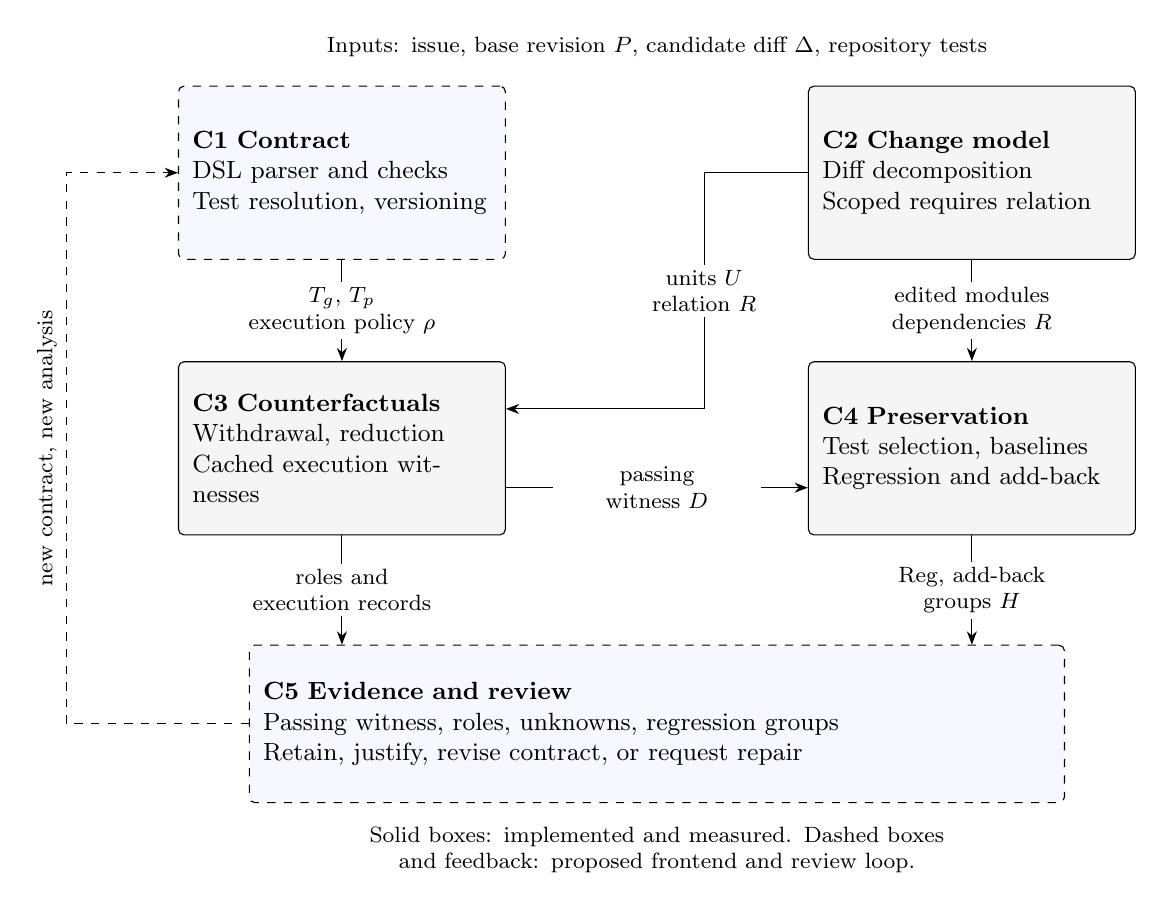
\begin{tikzpicture}[font=\small,>=Stealth,
 box/.style={draw,rounded corners=2pt,align=left,text width=38mm,minimum height=22mm,inner sep=5pt},
 proposed/.style={box,dashed,fill=blue!3},
 measured/.style={box,fill=black!4},
 lab/.style={font=\footnotesize,fill=white,inner sep=2pt,align=center}]
\node[proposed] (c1) at (0,0) {\textbf{C1 Contract}\\DSL parser and checks\\Test resolution, versioning};
\node[measured] (c2) at (8,0) {\textbf{C2 Change model}\\Diff decomposition\\Scoped requires relation};
\node[measured] (c3) at (0,-3.5) {\textbf{C3 Counterfactuals}\\Withdrawal, reduction\\Cached execution witnesses};
\node[measured] (c4) at (8,-3.5) {\textbf{C4 Preservation}\\Test selection, baselines\\Regression and add-back};
\node[proposed,text width=100mm,minimum height=20mm] (c5) at (4,-7.0) {\textbf{C5 Evidence and review}\\Passing witness, roles, unknowns, regression groups\\Retain, justify, revise contract, or request repair};
\draw[->] (c1.south) -- node[lab,text width=38mm]{$T_g$, $T_p$\\execution policy $\rho$} (c3.north);
\draw[->] (c2.south) -- node[lab,text width=32mm]{edited modules\\dependencies $R$} (c4.north);
\draw[->] (c2.west) -- (4.6,0) -- node[lab,text width=19mm]{units $U$\\relation $R$} (4.6,-3.0) -- ([yshift=5mm]c3.east);
\draw[->] ([yshift=-5mm]c3.east) -- node[lab,text width=25mm]{passing\\witness $D$} ([yshift=-5mm]c4.west);
\draw[->] (c3.south) -- node[lab,text width=28mm]{roles and\\execution records} (c3.south |- c5.north);
\draw[->] (c4.south) -- node[lab,text width=28mm]{$\operatorname{Reg}$, add-back\\groups $H$} (c4.south |- c5.north);
\draw[->,dashed] (c5.west) -- (-3.5,-7.0) -- node[font=\footnotesize,rotate=90,above]{new contract, new analysis} (-3.5,0) -- (c1.west);
\node[font=\footnotesize,align=center,text width=120mm] at (4,1.6) {Inputs: issue, base revision $P$, candidate diff $\Delta$, repository tests};
\node[font=\footnotesize,align=center,text width=120mm] at (4,-8.6) {Solid boxes: implemented and measured. Dashed boxes and feedback: proposed frontend and review loop.};
\end{tikzpicture}
\caption{Architecture and evidence flow. The current pipeline supplies C1's executable inputs directly, without a DSL parser. C4 also receives the contract's envelope policy $\eta$. In the retrospective study it inspects the reference patch to filter reference-observed test changes. A deployment would require explicit adjudication of such changes instead.}
\label{fig:architecture}
\end{figure}

The components address three distinct obstacles. Dependencies make arbitrary edit combinations hard to interpret, so C2 constrains the variants that C3 evaluates. Interacting edits make single removals insufficient, so C3 also searches for a passing subset. Incomplete tests leave preservation gaps, so C4 gathers additional observations. C1 and C5 give these mechanisms a stable behavioral interface rather than a list of preferred repair files.

For the running example, C1 supplies one goal test and 52 preservation tests. C2 produces four units with two dependency edges. C3 returns $D=\{u_3,u_4\}$ and witnesses for omitting $u_1$ and $u_2$. C4 checks 75 additional base-passing tests selected from database test modules. C5 would present the two-unit repair for focused review while keeping the omitted route and the observation boundary visible.

\subsection{C1: A language for behavioral intent}\label{sec:dsl}

The proposed language makes obligations reviewable before the agent's implementation is judged. Natural-language instructions often mix desired behavior, repair suggestions, and verification expectations. A contract separates these concerns. The language is deliberately small: it names executable observations and required evidence, without prescribing where a repair must be written.

Listing~\ref{lst:dsl} shows the contract for the example. Aliases resolve to exact test identifiers in a pinned test catalog. The preservation alias denotes the 52 tests described in Section~\ref{sec:running}. The envelope declaration requests up to six additional test modules using the implemented import-based selection policy. The repeat declaration applies to the full-patch stability check. The note records rationale and is not compiled into a test assertion.

\begin{lstlisting}[numbers=left,caption={Proposed \dsl{} contract. Test aliases are resolved before execution.},label=lst:dsl]
intent django_13297 {
  goal url_parameter {
    test catalog.template_params_filtering
  }
  preserve existing_views {
    tests catalog.generic_view_preservation
  }
  envelope import_rts top 6
  evidence full_repeats 2
  evidence counterfactual withdraw_and_reduce
  note "Wrapped URL values remain usable in queries"
}
\end{lstlisting}

The minimal syntax is as follows. A contract contains one or more named goal and preservation blocks, one envelope declaration, and both evidence declarations. Block names are unique. A \code{test} resolves to exactly one test, whereas \code{tests} resolves to a finite set. The optional note has no operational effect. Identifiers contain letters, digits, and underscores and begin with a letter. Catalog references are dot-separated identifiers. Integers use decimal notation, and strings are double-quoted text with escaped quotes and backslashes.
\begin{lstlisting}[numbers=none,basicstyle=\ttfamily\small,caption={Core grammar. Braces and quoted words are terminals.},label=lst:grammar]
Contract ::= "intent" Id "{" Goal+ Preserve+ Env Evidence Note? "}"
Goal     ::= "goal" Id "{" "test" TestRef "}"
Preserve ::= "preserve" Id "{" "tests" TestSetRef "}"
Env      ::= "envelope import_rts top" PositiveInt
Evidence ::= "evidence full_repeats" RepeatInt
             "evidence counterfactual withdraw_and_reduce"
Note     ::= "note" String
\end{lstlisting}

\paragraph{Static semantics.}
Compilation rejects any of the following: unresolved aliases, duplicate block names, a goal alias resolving to no test or to multiple tests, a nonpositive envelope size, fewer than two full-patch repetitions, and overlap between goal and preservation test identifiers. Requiring disjoint sets keeps the two roles unambiguous. Before a run, the base must reproduce the expected failing goal behavior and passing preservation behavior. A disagreement is a contract or environment diagnostic, not evidence about the submitted patch.

\paragraph{Execution semantics.}
Compilation produces $K=(T_g,T_p,\eta,\rho)$ together with the resolved catalog, base revision, and environment identifier. The fixed unknown-outcome policy records missing evidence and forbids interpreting it as a passing reduction or as a confirmed behavioral failure. The analysis records a digest of these inputs with the patch and all witness configurations. An agent may propose a contract amendment, but an amendment creates a new analysis identity and cannot weaken the obligations associated with earlier evidence. This separation matters when an agent also generates tests. The current study uses benchmark-defined obligations and therefore does not evaluate agent-authored contracts.

\begin{algorithm}[tbp]
\caption{Proposed contract compilation and preparation (C1)}\label{alg:compile}
\begin{algorithmic}[1]
\Require document $q$, catalog $A$, base $P$, environment $e$
\Ensure resolved contract and identity, or a diagnostic
\State $a\gets\Call{Parse}{q}$
\State \Call{CheckGrammarAndNames}{$a$}
\State $T_g\gets\Call{ResolveGoals}{a,A}$
\State $T_p\gets\Call{ResolvePreservation}{a,A}$
\State \Call{CheckCardinalityAndDisjointness}{$T_g,T_p$}
\State $\eta\gets\Call{ResolveEnvelope}{a}$
\State $\rho\gets\Call{ResolveEvidencePolicy}{a}$
\State \Call{CheckPolicyValues}{$\eta,\rho$}
\State $b\gets\Call{ExecuteBase}{P,T_g,T_p,e}$
\If{base expectations do not reproduce in $b$}
  \State \Return \Call{Diagnostic}{$b$}
\EndIf
\State \Return $(T_g,T_p,\eta,\rho),\Call{Digest}{P,e,A,a}$
\end{algorithmic}
\end{algorithm}

Algorithm~\ref{alg:compile} specifies the proposed frontend. Each check corresponds to one static-semantics rule above, and the final base execution enforces the reproduction requirement. The present analysis package does not implement parsing, diagnostics, digest management, or contract-edit authorization. An equivalent structured configuration could supply the same semantics. The empirical question is whether a dedicated language improves accurate authoring, comprehension, and maintenance of these contracts. Section~\ref{sec:future} defines that comparison instead of assuming that syntax alone yields a benefit.

\paragraph{Running example.}
The \code{url_parameter} block resolves to the exact reproduction test. The preservation block supplies stable view behavior, independently of the candidate's database edits. The maintainer's view repair and the agent's field-level repair can both satisfy the same contract. The abstraction therefore permits different implementations while requiring the same observable outcome.

\subsection{C2: Constructing a dependency-aware change model}\label{sec:decomposition}

C2 takes the base and candidate diff and returns $U$ and $R$. It locates each hunk by its preimage in the base, separates change runs, and reconstructs candidate variants from the unchanged revision. Agent edits to protected benchmark test files are excluded because the harness installs its own evaluation test patch. Other test and auxiliary-file edits remain visible, but their removability is interpreted separately from source-code behavior.

The implemented requires relation uses newly introduced or removed bindings. When an added use refers to a name that another unit newly binds, C2 records a requires edge. Conversely, when a unit removes a binding whose remaining uses another unit removes, the two are linked. Imports and assignments are matched within their module, because Python binds them per module. New functions and classes can establish cross-file edges through name-based matching. This is an approximate relation for Python. Dynamic imports, aliases, monkey patching, reflection, and implicit framework behavior can escape it. Conversely, name matching can add a spurious edge and force units to remain together. All guarantees are relative to the resulting admissible configurations.

Every constructed Python variant undergoes a parse check before test execution. A parse rejection avoids an expensive run, but it is not evidence that the withdrawn edit is behaviorally essential. Closed configurations can still fail at runtime because the dependency model is incomplete. The report records whether a rejection came from the precheck or from execution, so that these differences are not hidden behind a single semantic necessity claim.

\paragraph{Running example.}
The adapter branch $u_2$ uses the name that $u_1$ introduces, and the field branch $u_4$ uses the name that $u_3$ adds to an existing import. Thus
\[
R=\{(u_2,u_1),(u_4,u_3)\}.
\]
Although both providers import \code{LazyObject}, they bind it in different modules. Linking either branch to the other module's import would create a false dependency. An earlier implementation matched imports across files and made the unneeded import $u_1$ appear necessary. This case led to the per-module scoping rule, and all affected records were rerun. Withdrawing $u_3$ now removes $u_4$, while $u_1,u_2$ remain available. The recorded ablation without closure shows why the relation matters. It executed $\{u_4\}$ alone, which parses but references a name that is not bound. That run failed the goal test and all 52 preservation tests, an outcome caused by a broken variant rather than by behavioral necessity.

\subsection{C3: Counterfactual execution and witness reduction}\label{sec:triage}

C3 first checks that the full patch passes repeatedly and that the base does not already satisfy the goal. Repeats bypass the outcome cache. A nonreproducing full patch is outside the passing-patch analysis, and an unstable or unavailable outcome remains unresolved. Repeating the full patch does not establish that all subsets behave deterministically. Section~\ref{sec:rq4} measures repeated-configuration agreement directly.

The analysis then runs the permitted withdrawal of each unit from the full patch. It also invokes \textsc{ddmin}, accepting only variants that pass the core obligations~\citep{zeller2002ddmin}. Candidate subsets are closed under $R$ before evaluation. Because \textsc{ddmin} operates on generators whose closure can add units, its 1-minimality does not carry over to the closed result. A final pass therefore repeatedly removes a unit together with its dependents from the current closed witness whenever the resulting configuration passes. In Algorithm~\ref{alg:triage}, \textsc{FindPassingWithdrawal} enumerates these withdrawals in deterministic unit order and returns the first passing one, or \lab{none}. Unknown outcomes are recorded and never accepted as reductions.

\begin{algorithm}[tbp]
\caption{Dependency-aware counterfactual triage (C3)}\label{alg:triage}
\begin{algorithmic}[1]
\Require units $U$, relation $R$, contract oracle $\mathcal{O}_K$
\Ensure passing witness, contextual roles, and execution evidence
\State $b\gets\Call{CheckBaseAndRepeatedFull}{U,K}$
\If{$b$ does not establish the preconditions}
  \State \Return \Call{UnresolvedReport}{$b$}
\EndIf
\For{each $u\in U$}
  \State $o_u\gets\mathcal{O}_K(\withdraw_R(U,u))$
\EndFor
\State $D\gets\cl_R(\Call{DDMin}{U,\Valid_K\circ\cl_R})$
\State $W\gets\Call{FindPassingWithdrawal}{D,R,K}$
\While{$W\ne\lab{none}$}
  \State $D\gets W$
  \State $W\gets\Call{FindPassingWithdrawal}{D,R,K}$
\EndWhile
\State $L\gets\Call{AssignOperationalRoles}{D,\{o_u\}_{u\in U}}$
\State \Return $D,L,\Call{ExecutionEvidence}{K}$
\end{algorithmic}
\end{algorithm}

\textsc{AssignOperationalRoles} applies Definition~\ref{def:roles} to $D$ and $o_u$. The number of oracle executions is $n+O(n^2)$ in the worst case. The withdrawals contribute $n$, \textsc{ddmin} contributes $O(n^2)$, and the final pass contributes at most $n$ withdrawals per accepted reduction. In practice, caching and small patches keep the count low (Section~\ref{sec:rq4}). The cache avoids rerunning an identical configuration within a session, but it does not turn a nondeterministic test into a deterministic one. Cached outcomes are valid only for the same base, patch, contract, and environment. A deployed implementation would need to match these identities and adopt a deliberate stability policy before reusing outcomes across sessions.

\begin{proposition}[Passing witness and withdrawal minimality]\label{prop:minimality}
Assume a deterministic oracle, a closed valid full patch, and completed non-unknown outcomes for the final withdrawal neighborhood. Algorithm~\ref{alg:triage} returns a closed valid witness $D$ such that, for every $u\in D$, $\withdraw_R(D,u)$ is not valid.
\end{proposition}
\begin{proof}
The initial full patch is valid. Closure-aware \textsc{ddmin} and every accepted withdrawal preserve an observed valid closed configuration. Equation~\ref{eq:withdraw} removes a retained unit and all its dependents, so it yields a closed strict subset. Each accepted withdrawal therefore decreases the finite set $D$, and the loop terminates. At termination every permitted withdrawal has been considered and none is valid. Determinism and completed outcomes give the stated property.
\end{proof}

If a final withdrawal times out, the observed property is weaker: no tested withdrawal was accepted, but at least one possibility remains unknown. Such a run does not establish behavioral irreducibility. The records retain \lab{X} for unknown full-patch withdrawals, but they lack a separate certification flag for every uncertainty in the final neighborhood. We therefore report observed witness reductions rather than a certified guarantee for every empirical patch.

\begin{proposition}[Omission witness]\label{prop:omission}
For every unit $u\notin D$, the returned $D$ is a passing configuration that omits $u$. The complete omitted set $U\setminus D$ can therefore be removed together while preserving the observed core obligations.
\end{proposition}
\begin{proof}
The algorithm accepts a reduced configuration only after a valid outcome. Membership in $U\setminus D$ means that the corresponding unit is absent from that passing witness.
\end{proof}

These results are useful without implying global necessity or correctness. An \lab{N} withdrawal fails from the full patch, yet another repair subset might still omit that unit. An omitted edit can remain useful under an untested requirement. The output is an evidence-bearing review aid, not proof that the omitted changes are poor engineering.

\paragraph{Running example.}
Table~\ref{tab:example} lists the decisive configurations. The withdrawal outcomes and the passing witness yield \lab{U} for $u_1,u_2$ and \lab{N} for $u_3,u_4$. The run used eight oracle executions in total. Two were full-patch checks and one was the base check, four were withdrawals, and \textsc{ddmin} added one new configuration, $\{u_3\}$. The closure of $\{u_4\}$ is the cached witness, so that generator required no new run. The classification does not depend on proximity to the maintainer's view repair.

\begin{table}[pos=htbp]
\caption{Decisive running-example configurations (recorded). Every valid row also satisfies the 52 preservation obligations. The repeated full-patch run and the \textsc{ddmin} probe $\{u_3\}$ (goal-fail) are not shown.}
\label{tab:example}
\centering\small
\begin{tabular}{lll}
\toprule
Purpose & Retained units & Core outcome \\
\midrule
Base & $\emptyset$ & goal-fail \\
Full candidate & $u_1,u_2,u_3,u_4$ & valid \\
Withdraw $u_1$ and dependent $u_2$ & $u_3,u_4$ & valid \\
Withdraw $u_2$ & $u_1,u_3,u_4$ & valid \\
Withdraw $u_3$ and dependent $u_4$ & $u_1,u_2$ & goal-fail \\
Withdraw $u_4$ & $u_1,u_2,u_3$ & goal-fail \\
Witness $D$ & $u_3,u_4$ & valid \\
\bottomrule
\end{tabular}
\end{table}

The case has no retained alternative and no omitted withdrawal-sensitive unit. Two synthetic cases illustrate those roles without inventing repository results. If either of two edits independently repairs a defect, the retained one receives \lab{J}, because withdrawing it from the full patch leaves the other repair in place. If two compensating edits can be omitted together but not separately, the omitted units receive \lab{C}. These possibilities show that one-at-a-time deletion alone does not fully describe edit contribution. Section~\ref{sec:rq4} reports recorded instances of both roles.

\subsection{C4: Preservation beyond the core obligations}\label{sec:envelope}

Passing $T_g\cup T_p$ leaves behavior outside those tests unobserved. C4 therefore selects additional test modules using the candidate's actual edited source modules. The implemented import-based score combines direct imports, matching test filenames, package affinity, and proximity to the original test directories. It retains up to $k$ modules above a minimum score. This is a heuristic selection policy, not safe regression test selection, so its recall must be measured.

C4 runs the selected tests twice on the base and retains tests observed to pass both times. In the retrospective experiment it also runs the reference patch and excludes tests that fail there. This exclusion avoids automatically calling every reference-observed behavior change a regression, but it does not prove that the excluded behavior is intended. We therefore call the output a \emph{reference-filtered preservation signal}. A deployment without a reference patch would instead adjudicate the affected tests against the contract. An unavailable test result must remain unknown rather than count as a confirmed regression.

Let $T_E$ be the selected tests, $B$ the tests passing in both base runs, and $F(S)$ the completed failures on configuration $S$. Let $A$ contain tests excluded by the retrospective reference check or by explicit contract adjudication. The observed regression set is
\begin{equation}
\operatorname{Reg}(S)=\bigl(B\cap F(S)\bigr)\setminus(A\cup T_g).
\label{eq:regression}
\end{equation}
The implementation approximates this set by passing-set differences, which can also include unreported or interrupted tests. Every recorded regression was therefore re-executed in a fresh container, and only reproducing regressions are reported. The result remains subject to the harness's ability to distinguish failure from missing evidence.

If a regression disappears in $D$, C4 adds omitted units back to investigate it. An add-back can also include required support edits. Its observation implicates that closed group relative to $D$. It does not prove that one edit alone causes the failure in every context. Regressions already present in $D$ reveal a limitation of the core obligations that reduction cannot remove.

\begin{algorithm}[tbp]
\caption{Envelope observations and add-back witnesses (C4)}\label{alg:envelope}
\begin{algorithmic}[1]
\Require base $P$, full units $U$, relation $R$, witness $D$, policy $\eta$, exclusions $A$
\Ensure regression observations and implicated groups
\State $T_E\gets\Call{SelectAdditionalTests}{P,U,\eta}$
\State $B\gets\Call{StablePassingTests}{P,T_E}$
\State $G\gets\operatorname{Reg}(U)$ \Comment{Equation~\ref{eq:regression} on $T_E$}
\State \textbf{if} $G=\emptyset$ \textbf{then return} $\emptyset,\emptyset,\emptyset$
\State $G_D\gets\operatorname{Reg}(D)\cap G$
\State $H\gets\emptyset$
\For{each $u\in U\setminus D$}
  \State $S\gets\cl_R(D\cup\{u\})$
  \State $g\gets(G\setminus G_D)\cap\operatorname{Reg}(S)$
  \If{$g\ne\emptyset$} \State $H\gets H\cup\{(S\setminus D,g)\}$ \EndIf
\EndFor
\State \Return $G,G_D,H$
\end{algorithmic}
\end{algorithm}

Algorithm~\ref{alg:envelope} describes the intended evidence semantics. It requires two base runs, one full and one witness run when a regression occurs, and one add-back run per omitted unit. The existing add-back implementation adds the unit and its direct requirements rather than the full transitive closure, which differs only when requirement chains are longer than one edge. The \lab{H} tag in the records should therefore be read as an add-back association under that implementation, not as proof of isolated causal responsibility. Failures that arise only from interactions among several omitted groups can also escape individual add-backs.

\paragraph{Running example.}
C4 selects tests using the two database modules that the agent edited, even though the contract's original tests concern generic views. The selected modules include the base backend operation tests. The envelope contains 75 tests observed to pass on the base, and no envelope regression is recorded for the full candidate. Now suppose that a separately completed envelope test failed only after adding the omitted adapter route back to $D$. The report would then attach that test and the added group as a preservation witness. This hypothetical continuation explains the mechanism without converting an unobserved result into evidence.

\subsection{C5: Evidence for review and agent feedback}\label{sec:review}

The proposed report joins the resolved contract, unit definitions, requires edges, passing witness, withdrawal outcomes, and preservation observations. For each unit, it states whether the unit is retained, whether its full-patch withdrawal passes, and whether missing evidence limits the classification. It also records which additional tests were selected and which failures a reference-based rule excluded. An omission recommendation without these details would hide the conditions on which it depends.

The intended workflow offers three actions. A maintainer can review the passing witness first, retain an omitted edit with an explicit additional requirement, or request a repair when preservation fails. Adding a justified requirement changes the contract and triggers a new analysis. An agent can receive the same evidence and revise its patch, but its explanation does not replace the witness. The report does not delete logging, comments, defensive changes, or other edits merely because the current test suite does not require them.

\paragraph{Running example.}
The report would show $\{u_3,u_4\}$ as the passing core and $\{u_1,u_2\}$ as an omitted adapter route. A reviewer can ask whether adapter support is a separately desired requirement. If it is, that requirement needs its own executable evidence or explicit manual justification. The reduced patch still needs review for private-attribute access and untested lazy-evaluation behavior. In this way a higher-level contract governs different repair routes without equating minimality with engineering quality.

\section{Evaluation}\label{sec:evaluation}

\subsection{Research questions and setup}\label{sec:setup}

The evaluation tests whether the behavioral formulation yields information that location and whole-patch acceptance do not, while avoiding an unsupported claim that all agents behave less locally than humans. RQ1--RQ4 use completed analysis records. The DSL and review workflow have no measured results. Section~\ref{sec:future} specifies how to evaluate them. Table~\ref{tab:rqs} connects each question to its claim, evidence, and limits.

\begin{description}
\item[RQ1: Repair footprint.] Are recorded agent patches broader or more dispersed than the human reference patches for the same issues? This question tests the motivating premise.
\item[RQ2: Edit contribution.] What share of edits in resolved patches is removable under the benchmark obligations? Does it differ between agent and reference patches, and how closely do location heuristics and LLM judges approximate the counterfactual roles? This question tests whether contribution evidence is needed and available from cheaper signals (Contribution~1 and~3).
\item[RQ3: Preservation.] What additional behavior changes does the selected envelope expose, and what does a controlled injection study reveal about its limits? This question tests C4.
\item[RQ4: Cost, interaction, and reduction quality.] What execution cost does the analysis incur? How often do edit interactions arise? How close are the witnesses to minimum cardinality? This question tests C3 and Contribution~2.
\end{description}

\begin{table}[pos=htbp]
\caption{Question-to-evidence mapping. Agreement with operational labels is not independent validation of patch correctness.}
\label{tab:rqs}
\small\centering
\begin{tabularx}{\linewidth}{lXXX}
\toprule
Question & Evidence and comparison & Primary measurements & Interpretation boundary \\
\midrule
RQ1 & Paired agent/reference diffs, 46 systems; available trajectories & Size, dispersion, auxiliary files; rule: $\geq$2/3 of systems & One scaffold family; observational associations \\
RQ2 & Withdrawal and witness records; matched reference patches; proxies; five judges & Removable share and matched difference; precision, recall, MCC & Contribution relative to observed obligations \\
RQ3 & Additional tests; 500 mutation probes & Extra detections, observed failures, add-backs & Incomplete tests; possibly equivalent mutations \\
RQ4 & Execution records; ablations; exhaustive search for $\leq$8 units & Executions; \lab{C}/\lab{J} cases; minimum-cardinality agreement & Timing includes ablations; deterministic-oracle assumption \\
Planned & New controlled and longitudinal studies (Section~\ref{sec:future}) & Contract fidelity, held-out preservation, review accuracy & No results yet \\
\bottomrule
\end{tabularx}
\end{table}

\paragraph{Benchmark and sample.}
SWE-bench Verified supplies the base revisions, issue descriptions, tests, and reference patches. Public bash-only submissions provide candidate patches generated with the mini-swe-agent scaffold family~\citep{miniswe2025}. RQ1 includes the 46 systems with at least 450 patch files, which yields 22,954 agent patches across 500 instances. Paired footprint comparisons exclude 906 empty patches and use the remaining 22,048 agent--reference pairs. Holding the scaffold family broadly constant reduces one source of variation, but scaffold versions still differ, so we do not describe these runs as using an identical implementation.

The execution study uses Django and SymPy, which together contribute 306 of the benchmark's 500 instances. Ten instances require an unsupported execution architecture, and one further reference patch does not reproduce in the rebuilt environment. This leaves 295 validated instances. We analyze their reference patches and the officially resolved patches of the eight systems in Table~\ref{tab:panel}. Of 1,676 candidates, 1,674 reproduce the core resolution criterion. The two that do not, both from GPT-4o, are excluded from edit-role measurements.

\begin{table}[pos=htbp]
\caption{Execution panel and analysis coverage. Conclusive units exclude \lab{X}. All 20 unresolved units are source edits, spread across four agent patches.}
\label{tab:panel}
\centering\small
\begin{tabular}{lrrrr}
\toprule
System & Valid patches & All units & Conclusive units & \lab{X} \\
\midrule
Claude 4.6 Opus & 229 & 492 & 492 & 0 \\
GPT-5.2 high & 223 & 706 & 706 & 0 \\
Gemini 3 Pro high & 207 & 490 & 485 & 5 \\
Kimi K2.5 high & 222 & 470 & 463 & 7 \\
DeepSeek V3.2 high & 219 & 590 & 583 & 7 \\
GPT-5 mini & 174 & 314 & 313 & 1 \\
Qwen2.5-Coder 32B & 28 & 66 & 66 & 0 \\
GPT-4o & 77 & 286 & 286 & 0 \\
\midrule
Agent total & 1,379 & 3,414 & 3,394 & 20 \\
Reference patches & 295 & 914 & 914 & 0 \\
\bottomrule
\end{tabular}
\end{table}

\paragraph{Obligations and information access.}
The core analysis uses the instance's goal and preservation tests. These tests are visible to the analyzer, although they were withheld from the original repair agent. Once used for counterfactual search, they are not an independent evaluation oracle for the analyzer. The reference patch gives privileged information to the location proxies and to the retrospective envelope exclusion rule. Neither use is required for basic counterfactual reduction, but both limit claims about normal deployment.

\paragraph{Comparison methods.}
The reference-file proxy predicts that a source unit is retained when its file appears in the reference fix. The issue-mention proxy uses file and module names mentioned in the issue. Import proximity retains units within one import hop of reference-edited modules. The all-retained proxy represents accepting every unit. These rules approximate edit roles for diagnostic purposes and do not implement CIA in general. In particular, a reference-file proxy cannot substitute for evaluating a mature dynamic CIA or safe test-selection tool.

Five open-weight judges receive the issue and the same decomposed patch units: Gemma 2 9B, Llama 3.1 8B, Mistral Small 24B, Phi-4 14B, and Qwen2.5-Coder 7B. Each returns structured repair hypotheses and edit-role predictions. The main analysis aggregates parsed predictions over three seeds at temperature 0.2. A one-seed exploratory variant adds goal-test information. These comparisons measure agreement with execution-derived roles. The judges do not receive the execution feedback that \tool{} uses, so the results do not rank human-like review against execution-based methods in general.

\paragraph{Preservation probes.}
The injection study adds one unit to a reference patch in a nearby, previously unedited module. Semantic operators flip a relational operator, negate a condition, perturb an integer, or replace a return value with \code{None}. Neutral probes add a comment, redundant parentheses, or an unused assignment. The study contains 250 attempted probes of each category, drawn from eligible Django instances and a seeded sample of 30 SymPy instances. One execution per category ended in error, which leaves 249 evaluable probes per category. Mutation operators are useful sensitivity probes~\citep{jia2011mutation,just2014mutants}, but an undetected semantic mutation is not necessarily a behavioral fault, because it may be equivalent or unreachable under relevant inputs.

\paragraph{Analysis and decision rules.}
Edits are nested in patches and patches in instances. All intervals therefore resample instances (cluster bootstrap, percentile intervals, seed 2026), with 10,000 resamples for proportions and differences and 2,000 for classification metrics. RQ1 compares footprints with paired Wilcoxon signed-rank tests per system, Holm adjustment across systems within each metric, and matched-pairs rank-biserial effect sizes. The protocol, fixed before measurement, supports a general directional claim only if at least two thirds of systems (31 of 46) show a Holm-significant difference in the same direction. An exploratory logistic generalized estimating equation, clustered by instance with system fixed effects, relates footprint to resolution.

For RQ2, the positive class in precision, recall, and F1 is a removable unit (conclusive \lab{U} or \lab{C}), and MCC summarizes the retained/removable decision. Coverage and \lab{X} counts accompany these measures. The agent--reference comparison was added during this revision. It estimates the difference in removable share with instances resampled jointly, so that agent and reference units of the same instance stay together. Per-system comparisons restrict reference units to instances that the system resolved, which controls for the instances each system succeeds on. They report 95\% intervals, Bonferroni-adjusted intervals across the eight systems, and Holm-adjusted bootstrap $p$-values. The informed-judge comparison is likewise matched on seed and on units parsed in both variants. RQ3 compares official-test detection with detection by official tests plus envelope, using an exact McNemar test on the paired probe outcomes. RQ4 describes recorded executions and audits minimality against exhaustive search. The protocol records amendments made during implementation and execution, and analyses added in this revision are labeled as such. We do not describe the local protocol as independently preregistered.

\subsection{Implementation}\label{sec:implementation}

The measured pipeline is implemented in Python (about 1,600 lines for the analysis package). Its layers are patch decomposition and reconstruction, a scoped requires relation, counterfactual execution with caching and parse checks, import-based envelope selection, and result analysis. It consumes benchmark and structured configuration inputs directly. The \dsl{} parser, contract compiler, persistent evidence identity, and interactive review gate specified in Section~\ref{sec:approach} are not implemented components of this evaluation. There is consequently no measured result on language authoring or reviewer productivity. A suite of 121 unit and property-based tests checks decomposition, the requires relation, role assignment, \textsc{ddmin} 1-minimality, and agreement of the exhaustive baseline with brute-force enumeration on random oracles.

The oracle uses the SWE-bench 4.0.4 environment specifications, test commands, and log parsers. The study rebuilds the supported images for \code{linux/arm64}, and a reference-patch run validates each environment. For a candidate, a container starts from the pinned base, installs the protected benchmark test patch, and reconstructs every evaluated variant from that state. Test runs have a 900-second timeout, two assigned CPUs, 8\,GB of memory, and no network access. The full patch is executed twice before its edit roles are interpreted, and additional base runs support the envelope's stability filter.

The envelope ranks test modules by direct imports and matching filenames, each weighted three, package and original-test-directory affinity, each weighted two, and suitable parent-package imports, weighted one. Modules scoring at least two are eligible, and the six highest-ranking modules are selected. These choices define the evaluated heuristic and do not establish safe or complete test selection.

Patch execution took place on an Arm workstation with an NVIDIA GB10 and 121\,GB of memory. The judge models ran through node-local Ollama on NVIDIA H100 or A100 GPUs on the Rorqual and Narval clusters. The records retain requests, responses, seeds, timing, and model identities. The study used 27 Slurm jobs and 11.6 GPU-hours for 25,245 main judge responses. Reporting of model inputs and runtime choices follows recent guidance for LLM-based software engineering studies~\citep{baltes2027guidelines}.

Three implementation boundaries affect interpretation. First, the oracle's verdict layer can conflate some collection or load failures with obligation failures. Second, envelope add-backs use direct required units rather than the full closure. Third, the exhaustive-search ablation used in RQ4 originally enumerated configurations by their size before closure. Section~\ref{sec:rq4} reports how this defect was found, corrected, and accounted for. The formal design makes the first two distinctions explicit, and the results are interpreted according to the actual implementation.

\subsection{RQ1: Repair and exploration footprints}\label{sec:rq1}

Figure~\ref{fig:rq1} shows the per-system effects. The data do not support the motivating conjecture that agent patches are broader or more dispersed. Agents edit significantly fewer source files than the paired reference patches in 20 systems and more in six. They produce fewer source change blocks in 29 systems and more in one, and their edits are less dispersed in 22 systems and more dispersed in none. Source churn is mixed, with 14 systems higher and 11 lower. The median rank-biserial effects are $-0.31$ for source files, $-0.29$ for source blocks, and $-0.45$ for dispersion. Under the prespecified rule, however, none of these tendencies reaches the 31-system threshold. The closest case is source blocks, with 29 systems. The sample therefore supports neither ``broader'' nor, confirmatorily, ``more concentrated'' as a general property of agent patches.

\begin{figure}[pos=htbp]
\centering
%<<GEN:fig_rq1_effects>>
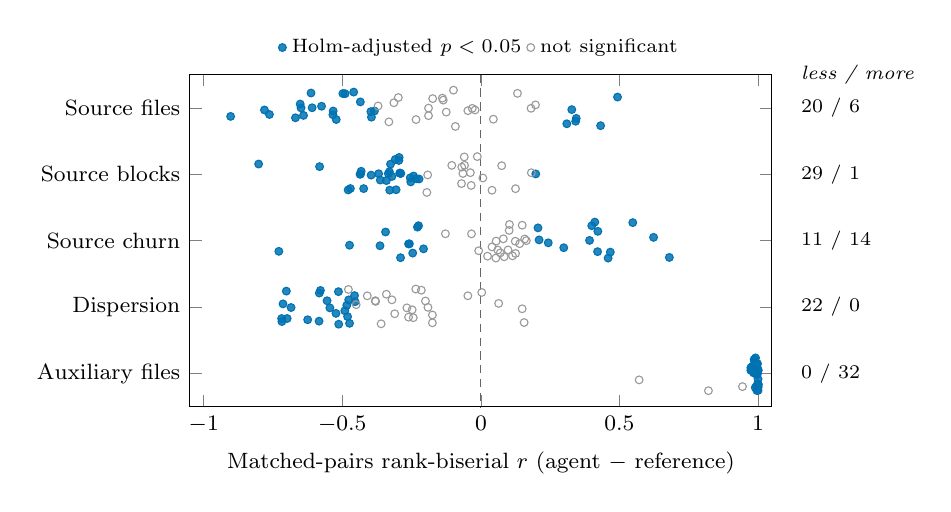
\begin{tikzpicture}
\begin{axis}[width=0.74\linewidth,height=58mm,xmin=-1.05,xmax=1.05,ymin=0.5,ymax=5.5,
 y dir=reverse,ytick={1,2,3,4,5},yticklabels={Source files,Source blocks,Source churn,Dispersion,Auxiliary files},xlabel={Matched-pairs rank-biserial $r$ (agent $-$ reference)},
 xtick={-1,-0.5,0,0.5,1},tick label style={font=\footnotesize},label style={font=\footnotesize},
 clip=false,legend style={font=\scriptsize,at={(0.5,1.02)},anchor=south,legend columns=2,draw=none}]
\addplot[only marks,mark=*,mark size=1.4pt,okblue,fill opacity=0.85] coordinates {(-0.490,0.787) (-0.649,1.001) (0.342,1.202) (-0.613,0.777) (-0.397,1.057) (0.344,1.159) (0.328,1.027) (-0.903,1.129) (-0.669,1.150) (-0.395,1.141) (-0.384,1.048) (-0.522,1.176) (-0.534,1.104) (-0.763,1.100) (0.493,0.838) (0.432,1.269) (0.310,1.240) (-0.459,0.763) (-0.435,0.911) (-0.781,1.032) (-0.575,0.976) (-0.640,1.114) (-0.652,0.943) (-0.533,1.048) (-0.609,0.999) (-0.498,0.785) (0.198,1.995) (-0.306,2.233) (-0.432,1.955) (-0.329,2.239) (-0.802,1.846) (-0.296,1.792) (-0.295,1.747) (-0.253,2.115) (-0.309,1.777) (-0.233,2.068) (-0.291,1.983) (-0.334,1.990) (-0.326,1.848) (-0.423,2.216) (-0.223,2.071) (-0.293,1.983) (-0.243,2.026) (-0.321,2.033) (-0.341,2.095) (-0.436,2.001) (-0.289,1.988) (-0.471,2.215) (-0.330,1.963) (-0.582,1.885) (-0.363,2.087) (-0.255,2.054) (-0.396,2.013) (-0.434,1.994) (-0.479,2.236) (-0.369,1.992) (0.467,3.172) (0.243,3.032) (-0.246,3.186) (0.400,2.775) (0.299,3.106) (-0.729,3.160) (0.459,3.262) (0.210,2.988) (-0.344,2.869) (-0.225,2.774) (0.623,2.950) (0.548,2.728) (0.411,2.720) (0.421,3.165) (0.422,2.859) (-0.474,3.068) (-0.290,3.256) (-0.364,3.076) (0.206,2.807) (-0.258,3.047) (0.680,3.252) (0.392,2.996) (-0.207,3.123) (-0.229,2.796) (-0.261,3.049) (-0.513,4.257) (-0.584,4.211) (-0.514,3.767) (-0.523,4.094) (-0.474,4.244) (-0.477,3.891) (-0.714,3.951) (-0.719,4.172) (-0.545,4.011) (-0.718,4.217) (-0.579,3.749) (-0.454,3.918) (-0.685,4.006) (-0.555,3.904) (-0.583,3.788) (-0.699,4.171) (-0.491,4.055) (-0.702,3.759) (-0.625,4.190) (-0.484,3.973) (-0.481,4.143) (-0.456,3.826) (0.990,5.212) (0.988,4.792) (0.996,5.017) (1.000,5.160) (0.996,5.009) (0.996,5.256) (0.987,4.810) (0.994,5.193) (1.000,4.938) (1.000,4.958) (0.974,4.952) (0.991,4.764) (0.979,4.891) (0.974,4.913) (0.996,4.868) (0.998,4.999) (1.000,5.157) (1.000,4.953) (0.987,4.982) (0.991,4.902) (0.984,4.990) (0.986,4.787) (1.000,5.166) (1.000,5.166) (1.000,5.177) (1.000,5.195) (0.998,4.850) (1.000,5.254) (1.000,5.212) (1.000,5.082) (0.977,4.948) (0.998,5.159)};
\addlegendentry{Holm-adjusted $p<0.05$}
\addplot[only marks,mark=o,mark size=1.4pt,okgrey] coordinates {(0.181,1.007) (-0.298,0.845) (-0.021,1.032) (-0.139,0.854) (-0.125,1.064) (0.132,0.782) (-0.234,1.177) (-0.371,0.972) (-0.174,0.861) (0.045,1.171) (-0.092,1.280) (-0.031,1.008) (-0.136,0.884) (-0.332,1.211) (-0.047,1.043) (-0.099,0.734) (-0.189,1.118) (-0.314,0.924) (0.197,0.956) (-0.189,1.004) (-0.070,2.140) (0.007,2.056) (-0.059,1.865) (-0.065,1.988) (-0.192,2.010) (-0.013,1.734) (0.125,2.217) (-0.038,1.976) (0.040,2.241) (-0.195,2.273) (-0.069,1.892) (-0.035,2.168) (0.075,1.871) (-0.060,1.739) (0.182,1.977) (-0.105,1.866) (0.055,3.006) (0.070,3.183) (0.114,3.228) (-0.034,2.897) (0.024,3.233) (0.124,3.008) (0.158,2.974) (0.054,3.261) (0.125,3.192) (0.103,2.756) (0.164,2.999) (0.098,3.139) (0.081,2.972) (0.140,3.045) (0.084,3.242) (0.149,2.767) (0.061,3.141) (0.040,3.094) (-0.128,2.896) (-0.008,3.151) (0.102,2.845) (-0.191,4.003) (-0.244,4.159) (0.156,4.232) (-0.410,3.830) (-0.235,3.728) (0.003,3.779) (-0.380,3.914) (-0.261,4.151) (-0.478,3.734) (-0.321,3.890) (-0.381,3.903) (-0.360,4.251) (-0.248,4.040) (-0.341,3.806) (-0.267,4.011) (-0.450,3.963) (-0.200,3.908) (-0.311,4.100) (0.064,3.944) (-0.047,3.829) (-0.175,4.236) (-0.215,3.745) (0.149,4.025) (-0.175,4.118) (0.944,5.196) (0.571,5.095) (0.821,5.258)};
\addlegendentry{not significant}
\draw[densely dashed,black!60] (axis cs:0,0.5) -- (axis cs:0,5.5);
\node[anchor=west,font=\scriptsize\itshape] at (axis cs:1.12,0.5) {less / more};
\node[anchor=west,font=\scriptsize] at (axis cs:1.12,1) {20 / 6};
\node[anchor=west,font=\scriptsize] at (axis cs:1.12,2) {29 / 1};
\node[anchor=west,font=\scriptsize] at (axis cs:1.12,3) {11 / 14};
\node[anchor=west,font=\scriptsize] at (axis cs:1.12,4) {22 / 0};
\node[anchor=west,font=\scriptsize] at (axis cs:1.12,5) {0 / 32};
\end{axis}
\end{tikzpicture}
%<<END:fig_rq1_effects>>
\caption{RQ1: per-system paired effects for 46 systems (22,048 non-empty pairs). Each point is one system. A negative $r$ means that the agent's patch is smaller or less dispersed than the reference patch for the same instance. Right margin: number of systems with a significant decrease / increase. A general directional claim requires 31 systems in one direction.}
\label{fig:rq1}
\end{figure}

Auxiliary files illustrate a scaffold confound. Thirty-two systems leave significantly more auxiliary files than the reference patches, which meets the threshold. None of the 14 mini-swe-agent 2.0 systems shows the difference, whereas earlier scaffold versions can include exploratory or reproduction files when extracting the submission. Attributing this effect to model reasoning would therefore be misleading.

Location still carries information at the system level. Across systems, resolution rate correlates negatively with mean nonlocal edit share (Spearman $\rho=-0.83$) and positively with the share of patches that touch a reference file ($\rho=0.94$). The second association is partly expected, because resolved patches usually modify the defective code. An exploratory instance-clustered model estimates an odds ratio of 0.34 for resolution per unit increase in nonlocal share, after adjustment for system, source churn, and edited-file count. This association does not show that a nonlocal repair is wrong, and the running example is a concrete counterexample to that reading.

The available trajectories show broader recorded search than final edits. Among the seven execution-panel systems with published logs, the median number of referenced repository files ranges from one to six, whereas the median final edit touches at most one file. A referenced file is extracted from shell-command text and serves as a proxy for recorded exploration. It does not prove that the agent read or understood every file. A human reference patch supplies no comparable exploration history.

\paragraph{Answer to RQ1.}
In this scaffold family, agent patches tend to be smaller and less dispersed than reference patches, but no directional difference is general enough to meet the prespecified criterion. The data provide no evidence of a universal human--agent difference in repair locality. The motivation for edit-level evidence therefore cannot rest on patch breadth. RQ2 tests whether it rests on edit contribution instead.

\subsection{RQ2: What the counterfactual witnesses reveal}\label{sec:rq2}

The 1,674 reproduced patches contain 4,328 units. Twenty units receive \lab{X}, which leaves 4,308 conclusive classifications. Among the 3,394 conclusive agent units, 62.0\% are \lab{N}, 0.3\% are \lab{J}, 1.9\% are \lab{C}, and 35.9\% are \lab{U}. The 914 reference units are 64.1\% \lab{N}, 2.0\% \lab{C}, and 33.9\% \lab{U}, with no \lab{J} units. These categories describe the selected witness and observed full-patch withdrawals, not global semantic necessity.

Among source units, 1,093 of 3,206 conclusive agent units are removable (34.1\%), against 328 of 914 reference units (35.9\%). The difference is $-1.8$ percentage points, with a 95\% interval of $[-8.6, 6.1]$. At least one removable unit of any kind appears in 30.1\% of agent patches (interval $[26.2\%, 34.0\%]$) and in 25.4\% of reference patches ($[20.7\%, 30.5\%]$). The pooled comparison mixes instance populations, because each system resolves a different subset of instances. Figure~\ref{fig:rq2} therefore compares each system with the reference patches of the instances it resolved. On those instances the reference share varies from 12.8\% (Qwen2.5-Coder) to 38.2\% (Claude 4.6 Opus), so instance composition alone moves the baseline substantially. DeepSeek V3.2 retains a higher removable share than its matched references ($+11.6$ points, $[4.3, 20.5]$, Holm $p=0.003$). GPT-4o shows a similar unadjusted difference ($+19.3$, $[4.4, 32.9]$, Holm $p=0.06$). The intervals of the remaining six systems include zero, and four of them point below the reference. The pooled matched difference is $-3.3$ points ($[-10.3, 5.4]$).

\begin{figure}[pos=htbp]
\centering
%<<GEN:fig_rq2_matched>>
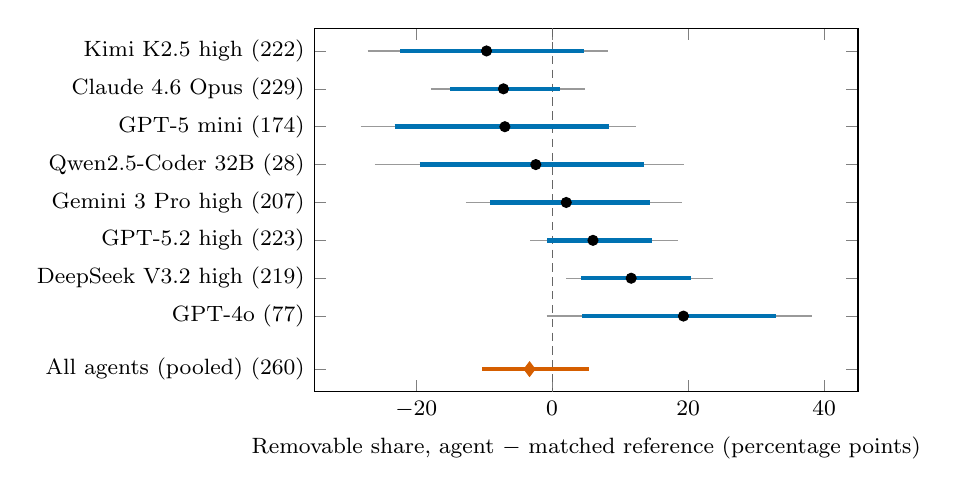
\begin{tikzpicture}
\begin{axis}[width=0.70\linewidth,height=62mm,xmin=-35,xmax=45,ymin=0.4,ymax=10.0,y dir=reverse,
 ytick={1,2,3,4,5,6,7,8,9.4},yticklabels={{Kimi K2.5 high (222)},{Claude 4.6 Opus (229)},{GPT-5 mini (174)},{Qwen2.5-Coder 32B (28)},{Gemini 3 Pro high (207)},{GPT-5.2 high (223)},{DeepSeek V3.2 high (219)},{GPT-4o (77)},{All agents (pooled) (260)}},xlabel={Removable share, agent $-$ matched reference (percentage points)},
 tick label style={font=\footnotesize},label style={font=\footnotesize},clip=false]
\draw[densely dashed,black!60] (axis cs:0,0.4) -- (axis cs:0,10.0);
\draw[okgrey,line width=0.5pt] (axis cs:-27.16,1) -- (axis cs:8.24,1);
\draw[okgrey,line width=0.5pt] (axis cs:-17.82,2) -- (axis cs:4.86,2);
\draw[okgrey,line width=0.5pt] (axis cs:-28.16,3) -- (axis cs:12.30,3);
\draw[okgrey,line width=0.5pt] (axis cs:-26.09,4) -- (axis cs:19.34,4);
\draw[okgrey,line width=0.5pt] (axis cs:-12.69,5) -- (axis cs:19.13,5);
\draw[okgrey,line width=0.5pt] (axis cs:-3.19,6) -- (axis cs:18.51,6);
\draw[okgrey,line width=0.5pt] (axis cs:2.07,7) -- (axis cs:23.62,7);
\draw[okgrey,line width=0.5pt] (axis cs:-0.82,8) -- (axis cs:38.19,8);
\draw[okblue,line width=1.6pt] (axis cs:-22.35,1) -- (axis cs:4.62,1);
\draw[okblue,line width=1.6pt] (axis cs:-15.04,2) -- (axis cs:1.23,2);
\draw[okblue,line width=1.6pt] (axis cs:-23.17,3) -- (axis cs:8.36,3);
\draw[okblue,line width=1.6pt] (axis cs:-19.51,4) -- (axis cs:13.56,4);
\draw[okblue,line width=1.6pt] (axis cs:-9.11,5) -- (axis cs:14.46,5);
\draw[okblue,line width=1.6pt] (axis cs:-0.74,6) -- (axis cs:14.76,6);
\draw[okblue,line width=1.6pt] (axis cs:4.32,7) -- (axis cs:20.50,7);
\draw[okblue,line width=1.6pt] (axis cs:4.41,8) -- (axis cs:32.87,8);
\addplot[only marks,mark=*,mark size=1.8pt,black] coordinates {(-9.65,1) (-7.16,2) (-6.95,3) (-2.40,4) (2.08,5) (6.01,6) (11.63,7) (19.32,8)};
\draw[okverm,line width=1.6pt] (axis cs:-10.28,9.4) -- (axis cs:5.41,9.4);
\addplot[only marks,mark=diamond*,mark size=2.6pt,okverm] coordinates {(-3.32,9.4)};
\end{axis}
\end{tikzpicture}
%<<END:fig_rq2_matched>>
\caption{RQ2: difference in removable share of conclusive source units between each system and the reference patches of the same instances (number of instances in parentheses). Thick bars: 95\% instance-cluster bootstrap intervals. Thin grey bars: Bonferroni-adjusted intervals across eight systems. Diamond: all agent units against the reference units of the 260 instances with at least one agent unit.}
\label{fig:rq2}
\end{figure}

Removable edits are thus common in both populations, and their prevalence depends more on the system and instance than on whether the author is human or agent. Passing-patch acceptance leaves the edit-level question open for all of them.

All 49 conclusive agent test-file units and 139 auxiliary-file units are removable under the benchmark obligations. This result reflects the harness, which protects its own test patch, and reproduction scripts typically lie outside the tested execution path. It does not imply that developer-written tests or debugging scripts have no engineering value.

Table~\ref{tab:comparisons} reports how well cheaper signals approximate the operational roles. Reference-file overlap flags removable edits with precision 0.83 but recall only 0.27. Of the 1,093 removable source units, 797 lie inside reference-edited files. Conversely, 60 retained source units lie outside those files, and the reference-file rule rejects all of them. Import proximity retains 63\% of these nonlocal retained units but finds only 21\% of removable units. Location therefore provides useful evidence but fails to distinguish many edits within the same repair area.

\begin{table}[pos=htbp]
\caption{Agreement with counterfactual roles for conclusive agent source units. Precision and recall concern removable units. Coverage is the share of 3,206 units with a parsed aggregate prediction. Intervals are 95\% instance-cluster intervals for MCC. The reference-file rule has privileged access to the reference patch.}
\label{tab:comparisons}
\centering\small
\begin{tabular}{lrrrrl}
\toprule
Method & Coverage & Precision & Recall & F1 & MCC [interval] \\
\midrule
Reference-file & 100\% & .83 & .27 & .41 & .37 [.26, .46] \\
Issue-mention & 100\% & .40 & .63 & .49 & .14 [.03, .24] \\
Import-proximity & 100\% & .91 & .21 & .34 & .35 [.24, .44] \\
All-retained & 100\% & -- & .00 & -- & -- \\
\midrule
Gemma 2 9B & 99.8\% & .77 & .16 & .27 & .25 [.19, .33] \\
Llama 3.1 8B & 98.3\% & .36 & .33 & .35 & .03 [$-$.05, .11] \\
Mistral Small 24B & 100\% & .91 & .29 & .44 & .42 [.34, .49] \\
Phi-4 14B & 98.5\% & .93 & .21 & .35 & .37 [.29, .44] \\
Qwen2.5-Coder 7B & 99.8\% & .52 & .37 & .43 & .22 [.13, .31] \\
\bottomrule
\end{tabular}
\end{table}

The best judge MCC is 0.42, for Mistral Small. Mistral Small and Phi-4 are precise when they predict removability, but their recall is only 0.29 and 0.21. The issue-mention rule has a higher F1 than any judge, although its MCC is lower. These metrics capture different tradeoffs and do not support a blanket claim that LLM judges outperform location. A matched exploratory comparison tests whether judges were handicapped by not seeing the goal tests. It uses the same seed and units parsed in both variants. The test information raises MCC for Phi-4 ($+0.07$, $[0.01, 0.15]$) and Qwen2.5-Coder ($+0.15$, $[0.02, 0.27]$), but not for Mistral Small ($-0.01$, $[-0.06, 0.03]$), Gemma, or Llama. The best informed MCC is 0.45. Test names and test code thus help weaker judges without closing the gap to the counterfactual measurement.

\paragraph{Answer to RQ2.}
Counterfactual witnesses identify a substantial removable portion of the tested patches, including many source edits inside reference-edited files. The removable share does not differ detectably between pooled agent and reference patches. It varies between systems, and one system exceeds its matched references after adjustment. Location heuristics and judges approximate the measurement only partly, even with test information. The result establishes a gap in evidence about edit contribution. It does not establish that removable edits are incorrect, or that the phenomenon is specific to agents.

\subsection{RQ3: Additional preservation evidence}\label{sec:rq3}

The selector finds an envelope for 1,636 valid patches and none for 38. The median nonempty envelope contains 104 tests observed to pass on the base. Confirmed reference-filtered envelope failures occur in 19 of 1,346 agent patches with nonempty envelopes (1.4\%, interval $[0.4\%, 2.7\%]$). In ten cases, add-back observations associate a failure with omitted units. In nine cases, the failure persists in the reduced witness, which shows that the core obligations permit a change that the envelope questions.

The records also contain two envelope signals for reference patches. A reference patch compared against its own reference-filtered baseline should not yield a stable difference. These signals point to repeated-execution effects, missing test reports, or baseline caching. They are not evidence of agent-specific regressions, and they caution against treating every envelope signal as a confirmed semantic defect. Re-execution reduces such uncertainty but cannot make the oracle complete.

Figure~\ref{fig:rq3} reports the controlled probes. Official tests detect 78 of 249 evaluable semantic probes (31.3\%, interval $[25.7\%, 37.3\%]$). The envelope detects another 25, which raises combined detection to 41.4\% ($[35.3\%, 47.4\%]$). The paired gain is 10.0 percentage points ($[6.4, 14.1]$), and all 25 discordant probes favor the envelope (exact McNemar $p<10^{-7}$). The remaining 146 semantic probes (58.6\%) are detected by neither. Detection depends strongly on the operator. Condition negation reaches 57.4\% combined detection, whereas integer perturbation reaches only 10.9\%, with one probe detected by the official tests and four more by the envelope. No neutral probe produced a test signal.

\begin{figure}[pos=htbp]
\centering
%<<GEN:fig_rq3_ops>>
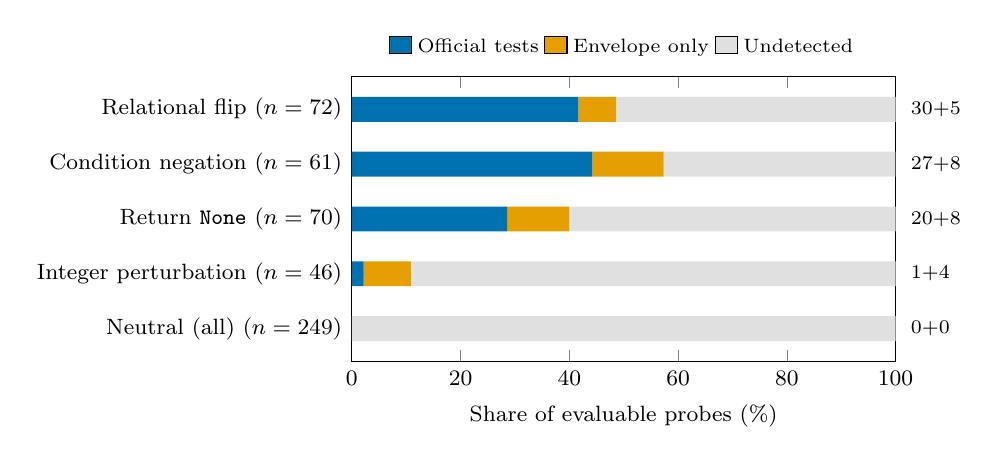
\begin{tikzpicture}
\begin{axis}[xbar stacked,bar width=9pt,width=0.70\linewidth,height=52mm,xmin=0,xmax=100,
 ymin=0.4,ymax=5.6,y dir=reverse,ytick={1,2,3,4,5},yticklabels={{Relational flip ($n=72$)},{Condition negation ($n=61$)},{Return \code{None} ($n=70$)},{Integer perturbation ($n=46$)},{Neutral (all) ($n=249$)}},
 xlabel={Share of evaluable probes (\%)},tick label style={font=\footnotesize},label style={font=\footnotesize},
 legend style={font=\scriptsize,at={(0.5,1.03)},anchor=south,legend columns=3,draw=none},clip=false]
\addplot[fill=okblue,draw=none] coordinates {(41.67,1) (44.26,2) (28.57,3) (2.17,4) (0.00,5)};
\addlegendentry{Official tests}
\addplot[fill=okorange,draw=none] coordinates {(6.94,1) (13.11,2) (11.43,3) (8.70,4) (0.00,5)};
\addlegendentry{Envelope only}
\addplot[fill=black!12,draw=none] coordinates {(51.39,1) (42.62,2) (60.00,3) (89.13,4) (100.00,5)};
\addlegendentry{Undetected}
\node[anchor=west,font=\scriptsize] at (axis cs:101,1) {30+5};
\node[anchor=west,font=\scriptsize] at (axis cs:101,2) {27+8};
\node[anchor=west,font=\scriptsize] at (axis cs:101,3) {20+8};
\node[anchor=west,font=\scriptsize] at (axis cs:101,4) {1+4};
\node[anchor=west,font=\scriptsize] at (axis cs:101,5) {0+0};
\end{axis}
\end{tikzpicture}
%<<END:fig_rq3_ops>>
\caption{RQ3: outcomes of injected probes by operator. Right margin: probes detected by official tests + additionally detected by the envelope. Detection means an observed test signal for a mutation probe, not independently established detection of a genuine fault. One erroneous execution per category is excluded.}
\label{fig:rq3}
\end{figure}

Zero observed neutral failures do not establish a zero population false-positive rate; with 249 probes, the one-sided 95\% upper bound is 1.2\%. Nor can every undetected semantic mutation be counted as a missed real fault without an independent behavioral witness. The measured quantity is sensitivity to the stated operator distribution and the selected sites. Integer perturbations, in particular, often change constants whose exact value no test constrains. A stronger study would distinguish killable faults, equivalent mutations, and mutations whose affected behavior lies outside the intended contract.

\paragraph{Answer to RQ3.}
Additional selected tests reveal behavior changes beyond the official obligations, with a statistically clear but modest gain. Most semantic probes remain undetected, particularly value perturbations, and add-back associations require contextual interpretation. A removable label must therefore remain relative to its contract and cannot serve as a certificate of harmlessness.

\subsection{RQ4: Cost, edit interaction, and reduction quality}\label{sec:rq4}

\paragraph{Cost.}
Core triage uses a median of three oracle executions per valid patch, with a 90th percentile of 11. Of the 1,674 patches, 877 contain one unit and another 376 contain two, so the overall median is dominated by small patches. Figure~\ref{fig:rq4} shows how executions grow with unit count (Spearman $\rho=0.97$). The median rises from 3 for one unit to 25 for 9--16 units and 66 for 17 or more, with a maximum of 256. The precheck rejects 79 configurations without a core test run. Across all valid patches, the median recorded wall time is 38.7 seconds. That timer starts before container execution and stops after optional ablations and the envelope. The timing values therefore do not establish a cost for the complete proposed workflow, or that one minimization method is faster than another under equal work.

\begin{figure}[pos=htbp]
\centering
%<<GEN:fig_rq4_cost>>
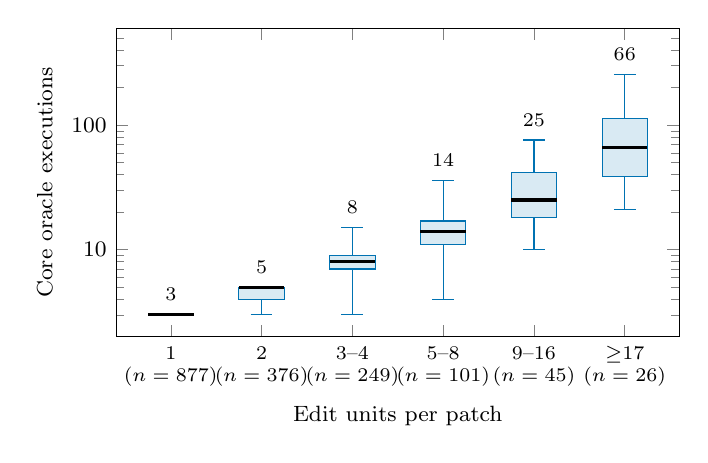
\begin{tikzpicture}
\begin{semilogyaxis}[width=0.72\linewidth,height=55mm,xmin=0.4,xmax=6.6,ymin=2,ymax=600,
 xtick={1,2,3,4,5,6},xticklabels={{1\\($n=877$)},{2\\($n=376$)},{3--4\\($n=249$)},{5--8\\($n=101$)},{9--16\\($n=45$)},{$\geq$17\\($n=26$)}},
 xticklabel style={align=center,font=\scriptsize},yticklabel style={font=\footnotesize},
 xlabel={Edit units per patch},ylabel={Core oracle executions},label style={font=\footnotesize},
 log ticks with fixed point,clip=false]
\addplot[draw=none] coordinates {(1,3)};
\draw[okblue] (axis cs:1,3) -- (axis cs:1,3);
\draw[okblue] (axis cs:1,3) -- (axis cs:1,3);
\draw[okblue] (axis cs:0.88,3) -- (axis cs:1.12,3);
\draw[okblue] (axis cs:0.88,3) -- (axis cs:1.12,3);
\draw[okblue,fill=okblue!15] (axis cs:0.75,3) rectangle (axis cs:1.25,3);
\draw[black,line width=1.2pt] (axis cs:0.75,3) -- (axis cs:1.25,3);
\node[font=\scriptsize,anchor=south] at (axis cs:1,3.24) {3};
\draw[okblue] (axis cs:2,3) -- (axis cs:2,4);
\draw[okblue] (axis cs:2,5) -- (axis cs:2,5);
\draw[okblue] (axis cs:1.88,3) -- (axis cs:2.12,3);
\draw[okblue] (axis cs:1.88,5) -- (axis cs:2.12,5);
\draw[okblue,fill=okblue!15] (axis cs:1.75,4) rectangle (axis cs:2.25,5);
\draw[black,line width=1.2pt] (axis cs:1.75,5) -- (axis cs:2.25,5);
\node[font=\scriptsize,anchor=south] at (axis cs:2,5.4) {5};
\draw[okblue] (axis cs:3,3) -- (axis cs:3,7);
\draw[okblue] (axis cs:3,9) -- (axis cs:3,15);
\draw[okblue] (axis cs:2.88,3) -- (axis cs:3.12,3);
\draw[okblue] (axis cs:2.88,15) -- (axis cs:3.12,15);
\draw[okblue,fill=okblue!15] (axis cs:2.75,7) rectangle (axis cs:3.25,9);
\draw[black,line width=1.2pt] (axis cs:2.75,8) -- (axis cs:3.25,8);
\node[font=\scriptsize,anchor=south] at (axis cs:3,16.2) {8};
\draw[okblue] (axis cs:4,4) -- (axis cs:4,11);
\draw[okblue] (axis cs:4,17) -- (axis cs:4,36);
\draw[okblue] (axis cs:3.88,4) -- (axis cs:4.12,4);
\draw[okblue] (axis cs:3.88,36) -- (axis cs:4.12,36);
\draw[okblue,fill=okblue!15] (axis cs:3.75,11) rectangle (axis cs:4.25,17);
\draw[black,line width=1.2pt] (axis cs:3.75,14) -- (axis cs:4.25,14);
\node[font=\scriptsize,anchor=south] at (axis cs:4,38.88) {14};
\draw[okblue] (axis cs:5,10) -- (axis cs:5,18);
\draw[okblue] (axis cs:5,42) -- (axis cs:5,76);
\draw[okblue] (axis cs:4.88,10) -- (axis cs:5.12,10);
\draw[okblue] (axis cs:4.88,76) -- (axis cs:5.12,76);
\draw[okblue,fill=okblue!15] (axis cs:4.75,18) rectangle (axis cs:5.25,42);
\draw[black,line width=1.2pt] (axis cs:4.75,25) -- (axis cs:5.25,25);
\node[font=\scriptsize,anchor=south] at (axis cs:5,82.08) {25};
\draw[okblue] (axis cs:6,21) -- (axis cs:6,38.75);
\draw[okblue] (axis cs:6,113.25) -- (axis cs:6,256);
\draw[okblue] (axis cs:5.88,21) -- (axis cs:6.12,21);
\draw[okblue] (axis cs:5.88,256) -- (axis cs:6.12,256);
\draw[okblue,fill=okblue!15] (axis cs:5.75,38.75) rectangle (axis cs:6.25,113.25);
\draw[black,line width=1.2pt] (axis cs:5.75,66) -- (axis cs:6.25,66);
\node[font=\scriptsize,anchor=south] at (axis cs:6,276.48) {66};
\end{semilogyaxis}
\end{tikzpicture}
%<<END:fig_rq4_cost>>
\caption{RQ4: core oracle executions per patch by number of edit units (log scale; box: interquartile range; whiskers: minimum and maximum; label: median). Executions include the two full-patch runs and the base run.}
\label{fig:rq4}
\end{figure}

\paragraph{Interactions.}
The records contain 82 \lab{C} units in 43 patches and nine \lab{J} units in seven patches. In these cases the full-patch single-withdrawal view and the selected passing witness disagree. A procedure that treated every failed single withdrawal as global necessity would keep the omitted withdrawal-sensitive edits. These observations motivate reporting both the full-patch experiment and the reduced witness.

\paragraph{Reduction quality.}
For the 1,603 patches with at most eight units, an ablation searched exhaustively for minimum-cardinality closed configurations. Our first comparison found the exhaustive minimum larger than a known passing witness in four records, which is impossible for a correct exhaustive search under a deterministic oracle. An audit traced the cause to the baseline, not to \tool{}. The baseline enumerated subsets by their size before closure. A small generator whose closure was large, such as two units whose closure was the whole patch, was returned before a smaller valid closed set was reached. All four records contain requires edges, and in each the smaller \tool{} witness had itself been observed valid. We corrected the enumeration to order closed configurations by their own size and added regression and property-based tests. The original code fails the regression case and 9 of the 40 random cases. We then re-derived the minimum from the recorded outcomes. For 1,595 records, every closed configuration smaller than the witness has a recorded or static-precheck non-valid outcome. For seven records, 31 smaller closed configurations had never been executed. We executed them, together with one re-execution of each witness. All 31 failed and all seven witnesses passed again. One record (\code{sympy__sympy-19783}, Kimi K2.5) has a valid two-unit closed configuration, whereas \tool{}'s witness has three units. This is the expected gap between withdrawal minimality and minimum cardinality. Overall, 1,602 of 1,603 witnesses (99.9\%) have minimum cardinality among closed configurations. Matching size establishes neither uniqueness of the minimal repair nor stability of every edit label.

These conclusions assume deterministic outcomes, which we checked directly. The records execute 3,746 configurations more than once, through repeated full-patch checks and ablation reruns. Two of them, in \code{django__django-16263} (reference) and \code{sympy__sympy-13091} (Kimi K2.5), produced conflicting outcomes. Both patches have more than eight units, and their labels inherit that instability. Nondeterminism is therefore rare (0.05\% of repeated configurations) but present.

The other ablations compare plain reduction, precheck-only reduction, dependency-aware reduction, and leave-one-out. They reuse available outcomes and execute additional configurations when needed, and their output requirements differ. Full triage produces withdrawal evidence as well as a passing subset, while a minimizer can stop after obtaining the subset. Raw call totals therefore do not isolate the cost of the same task. A fair head-to-head comparison requires common information, output requirements, and budgets (Section~\ref{sec:future}).

\paragraph{Answer to RQ4.}
Core counterfactual execution is inexpensive for the predominantly small patches in this sample and grows steeply for large ones. Interaction cases justify evidence beyond leave-one-out. Although \tool{} guarantees only withdrawal minimality, its witnesses attain minimum cardinality in all but one of 1,603 exhaustively checked patches. The existing timing instrumentation does not isolate end-to-end governance cost.

\subsection{Planned evaluation of the contract workflow}\label{sec:future}

The implemented analysis does not establish the benefits of a DSL or of integrating evidence into agent development. We propose three complementary studies. Each has a primary outcome and a result that would weaken the proposed approach. These studies are future work, not completed experiments.

\paragraph{Study A: language value and contract fidelity.}
Compare natural-language instructions, an equivalent structured YAML configuration, and \dsl{} in a balanced crossover design with software developers. Each participant writes and amends goal and preservation policies for different tasks under each interface. An expert-authored mapping from requirements to tests, prepared before the sessions, serves as the reference. The primary outcome is the rate of contracts that express all required obligations without adding contradictory ones. Secondary outcomes are authoring time, diagnostic recovery, comprehension, and amendment errors. A pilot estimates variance to set the confirmatory sample size for a prespecified effect or interval width. A null advantage over equivalent YAML would weaken the claim that dedicated syntax improves governance, while leaving the underlying contract model useful.

\paragraph{Study B: equal-budget analysis and review.}
Freeze a new task set and its candidate patches before any tuning. Compare unchanged patches, leave-one-out, dependency-aware \textsc{ddmin}, a structure-aware reducer, TRIM, and \tool{}. TRIM is the most important comparison because it also uses counterfactual execution and reports about half the validation cost of delta debugging~\citep{mathai2026trim}. Supply trajectories where available and report a separate diff-only stratum where they are not. Use identical analyzer-visible tests, clean environments, and equal test-execution or wall-time budgets. Measure witness size, retained held-out behavior, unresolved outcomes, and total execution cost, and evaluate attribution evidence separately from plain minimization. This design can reveal whether the added evidence is worth its cost, rather than assuming that a richer report is better.

For independent preservation assessment, prepare evaluation-only tests or adjudicated behavioral checks that the analyzer cannot access. Keep reference-patch information out of the deployed method and use it only for explicitly privileged diagnostics. Independent reviewers inspect a stratified sample of retained, omitted, and unresolved units with the issue context. A blinded crossover review task then compares ordinary diffs with the evidence report. The primary review outcome is correct acceptance or rejection under an adjudicated requirement set. Review time is secondary, because a faster incorrect decision is not an improvement. If reduced patches lose held-out behavior or the evidence increases confident review errors, the workflow must be revised.

\paragraph{Study C: cumulative development and wider applicability.}
Use the version-pinned benchmark roles in Table~\ref{tab:benchmarks}. SWE-bench Verified remains the primary repair benchmark because it supplies repository tasks, reproducible environments, and archived candidate patches. Defects4J provides a Java replication setting~\citep{just2014defects4j}, for which the dependency model must be adapted and validated rather than transferred mechanically from Python. SlopCodeBench supplies successive specification updates for studying how earlier agent changes affect later development~\citep{orlanski2026slopcodebench}. Its exact release must be frozen, because the paper and repository have changed across versions.

In the iterative study, each accepted implementation is carried into the next task. Compare ordinary agent iteration with contract-and-evidence feedback under matched generation and validation budgets, and hold later checkpoint tests out of earlier feedback. The primary outcome is successful completion of subsequent requirements while preserving prior required behavior. Secondary outcomes include repair churn, redundant structure, new contract obligations, and cumulative execution cost. If a smaller initial patch makes later changes harder, that would challenge minimality as a review objective.

\begin{table}[pos=htbp]
\caption{Recommended benchmark roles for the remaining evaluation. Only the SWE-bench Verified execution subset has been analyzed in the results reported here.}
\label{tab:benchmarks}
\centering\small
\begin{tabularx}{\linewidth}{lXXX}
\toprule
Benchmark & Why it fits & Required preparation & Main limitation \\
\midrule
SWE-bench Verified & Real issue repair, candidate patches, executable obligations & Freeze snapshots; audit environments and hidden evaluation split & Public tests and reference history may be contaminated \\
Defects4J & Reproducible real Java faults and regression suites & Obtain agent candidates; validate Java unit dependencies & Curated human fixes alone do not test agent behavior \\
SlopCodeBench & Repeated implementation under evolving requirements & Freeze release; preserve trajectories; hide future tests & Different task construct from repository bug repair \\
\bottomrule
\end{tabularx}
\end{table}

All three studies should report information access, failures, model and scaffold versions, and full denominators. A contract-generated test and a held-out evaluator test must not silently become the same evidence source. A question counts as answered only when its stated construct has been measured, not merely because a benchmark score improves.

\subsection{Discussion}\label{sec:discussion}

\paragraph{The deeper problem is an evidence mismatch.}
The starting intuition was that an agent may analyze and repair software differently from a particular human developer. The data support a narrower and more useful conclusion: neither a reference repair location nor a passing whole patch establishes the contribution of every candidate edit. RQ1 finds no general breadth difference in this sample, and RQ2 finds many removable edits inside reference-edited files. Governance based only on edit radius would miss those cases. Governance based on explicit obligations asks the relevant question without requiring a cognitive theory of agents.

\paragraph{Why counterfactual witnesses succeed where cheaper signals fail.}
Location proxies and judges observe where an edit is and what it looks like. A withdrawal experiment observes what happens without the edit. Most removable source edits lie in the same files as the reference repair (797 of 1,093). They are typically defensive branches, symmetric cases, or duplicate routes next to the effective change, so location cannot separate them. Test information helps some judges (RQ2), which suggests that their errors partly reflect missing knowledge of the obligations. Even informed judges reach an MCC below 0.5, however, so predicting execution outcomes from text remains hard. The counterfactual witness is more expensive, but RQ4 shows that the expense is small for typical patches.

\paragraph{Human patches expose the oracle's limits.}
Reference and agent patches show similar pooled source-unit removability, which rules out an agent-specific interpretation of the overall result. The system-level differences show that some agent configurations leave more removable code than the corresponding human fixes, while others leave less. Maintainers add symmetric fixes, defensive branches, and readability improvements that the benchmark does not exercise. An analyzer that calls these units removable may describe the test suite accurately but the engineering task incompletely. This is why the reference comparison matters: it shows that relevance cannot be defined solely by human location or by test necessity.

\paragraph{Alternative repair routes deserve evidence, not automatic rejection.}
Location is informative across systems, but it is not a correctness rule for an individual repair. The running example demonstrates a nonlocal route that passes the obligations, with both retained and omitted edits along that route. A behavioral contract admits that possibility. Counterfactual success does not, however, excuse a design that violates an untested requirement. The appropriate response is to make that requirement explicit and gather more evidence.

\paragraph{Preservation signals should drive refinement, not certification.}
The envelope's additional detections show why reduction and preservation checks belong together. The large undetected fraction, concentrated in value perturbations, shows why they are insufficient as a safety claim. A failure in the reduced witness calls for stronger obligations or a revised repair. A failure associated with omitted units focuses review on those groups. The proposed report should make both cases visible, including tests excluded by the retrospective reference rule.

\paragraph{Relation to trajectory-based minimization.}
TRIM already studies execution-based removal of residual agent changes and reports substantial reductions at about half the validation cost of delta debugging~\citep{mathai2026trim}. Counterfactual patch minimization is therefore not new. Our RQ4 result suggests that, for the small patches typical of this benchmark, a final-diff analysis with a dependency relation already reaches minimum cardinality almost always. Trajectory guidance may matter most for the cost of large patches, where executions grow steeply. The distinct elements of \tool{} are the explicit behavioral contract, the separation of contextual roles from global necessity, and preservation observations attached to omitted groups. TRIM also reports that agent code tends to be larger than human code, whereas our RQ1 finds no general difference. The constructs differ in scaffolds, tasks, and size measures, so the two results do not directly contradict each other. Whether the additional evidence improves development outcomes remains an empirical question, which Study~B makes falsifiable.

\paragraph{Auditing a baseline is part of the evidence.}
The exhaustive-search defect shows how a reduction comparison can fail silently once a dependency closure is involved. The faulty baseline agreed with \tool{} in 99.7\% of records and disagreed only where requires edges existed. Without the audit, these disagreements would have read as either a flaw in \tool{} or an unexplained anomaly. Generators and their closures are easy to conflate, and the same pitfall applies to any closure-aware reduction. Evaluations of such methods should check their baselines against brute-force enumeration over closed sets.

\paragraph{A review aid is not an automatic merge policy.}
The most defensible near-term use is to expose a passing repair core and the evidence for omitted groups. A maintainer may retain additional edits for a documented reason. Automatic deletion would elevate incomplete test evidence above requirements that the tests do not represent. The workflow should support asking for the missing requirement rather than hiding the uncertainty behind a categorical label. The contract language moves review from preferred files to explicit behavior and evidence requirements, but it cannot determine whether the obligations faithfully represent user intent. Study~A is needed because an equivalent structured configuration may offer the same practical benefit with less language machinery.

\subsection{Threats to validity}\label{sec:validity}

\paragraph{Construct validity.}
Edit roles measure contract-relative observations and membership in one selected witness. They do not measure complete relevance, maintainability, or human reasoning. Name-based dependencies can merge unrelated units or miss dynamic relations. The current harness does not always separate structural from behavioral rejection. Reference-file proxies are narrow diagnostic rules, not comprehensive CIA baselines. Mutation probes measure sensitivity to specified transformations, not a ground-truth sample of real regressions. Referenced files in trajectories are a textual proxy for exploration. These boundaries restrict what each reported number means.

\paragraph{Internal validity.}
Full-patch repetition and repeated base-envelope runs reduce flakiness but do not eliminate it. Two of 3,746 repeated configurations disagreed, so a cached single outcome can occasionally fix an unstable label. A counterfactual can activate a path that the full patch does not exercise. Reference-filtered set differences can confuse missing reports with failures, which re-execution mitigates. The 20 unresolved units are excluded from denominators. Two method corrections were made during execution, closure-aware reduction and per-module scoping, and affected records were rerun under the protocol amendments. The exhaustive baseline defect was corrected after the main runs. Its effect was reanalyzed from recorded outcomes, and only the missing configurations were newly executed. The original records were preserved.

\paragraph{External validity.}
Execution covers 295 instances from two Python projects, eight model systems, and one scaffold family. Resolved-only selection excludes unsuccessful repair attempts and cannot estimate their relevance distribution. Architecture-based exclusions can favor reproducible tasks. Systems resolve different instance subsets, which the matched comparison addresses only for removability. Results may differ for industrial repositories, other languages, richer scaffolds, configuration changes, and long development histories. Public benchmark data may also be contaminated in model training. This affects which patches were produced, but not the execution-based measurements of those patches.

\paragraph{Conclusion validity.}
Edits are nested in patches and issues, so all intervals resample instances. Samples remain unbalanced across systems, and Qwen2.5-Coder and GPT-4o contribute few instances. Per-system comparisons use multiplicity-adjusted intervals and $p$-values, but the other analyses report unadjusted 95\% intervals as descriptive uncertainty. Judge metrics are conditional on parsed predictions and conclusive labels. The best judge is selected from a small panel, and the informed variant is exploratory. The agent--reference comparison was added during this revision rather than prespecified. Cost comparisons require matching both work and output, which the existing ablations do not do.

\paragraph{Research status and reproducibility.}
The results come from the recorded execution campaign, its processed artifacts, and the revision analyses listed in the data availability statement. The formal properties describe the stated design under explicit assumptions. The DSL compiler and review loop remain proposed. An immutable archival deposit of the replication package is still required.

\section{Related work}\label{sec:related}

Table~\ref{tab:related} summarizes how \tool{} relates to the closest families of techniques. The comparison concerns the problem each family addresses, its inputs and outputs, and the guarantee it provides. It is not a ranking.

\begin{table*}[pos=htbp]
\caption{Positioning against the closest technique families. Entries summarize the cited work's stated problem and outputs.}
\label{tab:related}
\centering\footnotesize
\begin{tabularx}{\textwidth}{>{\raggedright\arraybackslash}p{27mm}*{4}{>{\raggedright\arraybackslash}X}}
\toprule
Family & Question answered & Main inputs & Output & Guarantee or evidence \\
\midrule
CIA and Chianti~\citep{li2013cia,ren2004chianti} & What may a change affect? & Program, change, dependencies, tests & Affected elements or tests & Sound or approximate dependence; no requirement on the change \\
Regression test selection~\citep{rothermel1997safe,gligoric2015ekstazi} & Which tests must be rerun? & Change, dependency or coverage data & Test subset & Safety under stated assumptions \\
Delta debugging, HDD~\citep{zeller2002ddmin,misherghi2006hdd} & Which smaller input preserves an outcome? & Configuration set, test function & One reduced configuration & 1-minimality \\
Change untangling~\citep{herzig2013tangled,barnett2015untangle,dias2015untangling} & Which changes belong together? & Commit or changeset & Partition of changes & Heuristic grouping for comprehension \\
TRIM~\citep{mathai2026trim} & Which agent edits are search leftovers? & Agent trajectory, final patch, tests & Reduced patch & Execution-validated reduction \\
Patch correctness assessment~\citep{qi2015kali,wang2020apr} & Does a plausible patch overfit? & Patch, tests, sometimes reference & Correct or overfitting verdict & Empirical, per patch \\
\tool{} (this paper) & Which edit groups does a stated contract require, and what is observed beyond it? & Final diff, contract, environment & Witness, roles per unit, envelope regressions with add-back groups & Withdrawal minimality; omission witnesses; observed only \\
\bottomrule
\end{tabularx}
\end{table*}

\subsection{Impact analysis, localization, and regression selection}

CIA identifies the potential effects of code changes through structural and execution dependencies~\citep{bohner1996cia,li2013cia,orso2003field}. Chianti is an important precedent: it decomposes a change into atomic changes and relates them to tests~\citep{ren2004chianti}. Regression selection uses dependency evidence to avoid unnecessary test execution, with safety guarantees under defined assumptions~\citep{rothermel1997safe,gligoric2015ekstazi}. Fault localization ranks code associated with a failure~\citep{wong2016fl}. None of these problem definitions requires that the author be human, and all of them remain applicable to agent patches.

\tool{} differs in its main output. It asks which groups of a given passing patch can be omitted while preserving specified outcomes, and it records witnesses for that judgment. It reuses dependency analysis and regression selection rather than replacing them, and a stronger dynamic or safe selection method could improve C4. Our reference-location comparisons should therefore be read as evidence about location proxies, not as a comprehensive comparison with CIA techniques.

\subsection{Program repair and patch correctness}

Generate-and-validate repair accepts candidates that meet executable checks~\citep{legoues2012genprog}. Semantics-based methods synthesize changes from constraints~\citep{nguyen2013semfix,mechtaev2016angelix}. The repair literature has long distinguished plausible from correct patches and documented overfitting to the available tests~\citep{qi2015kali,smith2015cure,wang2020apr}. Recent work examines how model and fine-tuning choices affect repair capability~\citep{huang2025comprehensive}. GiantRepair combines LLM-provided changes with program analysis and synthesis~\citep{li2025hybrid}. Work on Alloy repair evaluates model and feedback configurations for declarative specifications~\citep{alhanahnah2025specifications}.

These studies improve patch generation or assess the correctness of its result. \tool{} starts from a candidate and describes its internal contribution structure under explicit obligations. A passing reduced patch can still overfit, so correctness assessment remains complementary. The contract language neither confers semantic correctness on tests nor replaces a formal specification language such as Alloy. It organizes the observations and evidence that a development workflow requires.

\subsection{Reduction, residual agent edits, and change untangling}

Delta debugging provides the central counterfactual reduction mechanism~\citep{zeller1999yesterday,zeller2002ddmin}, and hierarchical reduction uses structure to avoid invalid candidates~\citep{misherghi2006hdd}. Change-untangling research shows that human commits mix concerns, and it groups changes to support comprehension and review~\citep{herzig2013tangled,barnett2015untangle,dias2015untangling}. These precedents caution against attributing mixed-purpose changes exclusively to agents, which our reference-patch results confirm.

TRIM is the closest recent approach. It reconstructs agent edit histories and uses their temporal order to approximate dependencies during a hierarchical counterfactual search~\citep{mathai2026trim}. \tool{} works from the final diff with a static requires relation, which applies when trajectories are unavailable but may miss dependencies that the trajectory would reveal. Its output includes contract-relative edit roles and preservation observations, not only a smaller passing patch. Both approaches use execution-based omission, and neither can establish untested behavior from a passing suite. We claim no superiority over TRIM without the equal-budget comparison of Study~B. Trajectory ordering could also be combined with \tool{}'s evidence model.

\subsection{Agent behavior, benchmarks, and behavioral governance}

SWE-bench and SWE-bench Verified make repository repair measurable~\citep{jimenez2024swebench,chowdhury2024verified}. SWE-agent, Agentless, and mini-swe-agent explore different organizations of tool interaction and repair~\citep{yang2024sweagent,xia2025agentless,miniswe2025}. Trajectory studies investigate observable thought--action--result patterns~\citep{bouzenia2025trajectories}. PAGENT analyzes failed patches and uses program analysis to address type-related errors~\citep{xue2025pagent}. SlopCodeBench moves evaluation toward successive changes and the code that later tasks inherit~\citep{orlanski2026slopcodebench}.

These studies motivate the task setting and possible failure mechanisms, but they do not make imitation of the reference route an adequate governance policy. \tool{} connects a candidate's changes to explicit obligations and omission witnesses. The proposed language brings a contract perspective to that workflow~\citep{meyer1992dbc}, but its authoring and review benefits remain to be established. Recent reporting guidance supports documenting model inputs, analysis decisions, and artifact provenance~\citep{baltes2027guidelines}. That guidance informs reproducibility, not the effectiveness of a particular technique.

\section{Conclusion}\label{sec:conclusion}

Agent-generated patches should be judged against intended behavior and preservation requirements, while alternative implementation routes remain admissible. \tool{} operationalizes this principle through dependency-aware counterfactual execution, a passing witness subset, contextual edit roles, and additional regression observations. The proposed \dsl{} language gives the behavioral contract an explicit form above the level of repair locations.

The evidence does not support a general claim that agent patches are broader than human patches. It does show that passing patches from both sources contain source edits that the benchmark obligations do not require. The prevalence of such edits varies more across systems and instances than between humans and agents, and location proxies and LLM judges miss many of them. Additional tests expose some unobserved behavior changes but leave substantial uncertainty. The witnesses reach minimum cardinality in all but one exhaustively checked patch, a result that required correcting the baseline used to check them. The next empirical steps are an implementation of the contract language and review workflow, an equal-budget comparison with trajectory-based minimization, and evaluation with independent preservation checks and successive development tasks.

\section*{Data availability}
The SHIFT project contains the implementation, protocols, per-patch execution records, analysis scripts, and the revision analyses: the exhaustive-search audit (\nolinkurl{analysis/revision/exhaustive_audit.py}), its follow-up executions (\nolinkurl{experiments/revision_exhaustive_followup.py}), the revision statistics (\nolinkurl{analysis/revision/revision_stats.py}), and the figure generator (\nolinkurl{analysis/revision/figures.py}). Every figure in Section~\ref{sec:evaluation} is generated from the processed tables by that script. The project's version-control remote is \url{https://github.com/ai4se4ai-lab/SHIFT}. This revision did not verify the public availability or completeness of that remote, and no immutable archival release has yet been made. The planned studies have no results or participant data.

\section*{Declaration on the use of AI}
An earlier manuscript version reports AI assistance in research software development, experiment execution, and writing. A previous revision used OpenAI Codex to assist with literature inspection, local artifact checks, technical exposition, and drafting. This revision used Claude Code (Anthropic) to audit the analysis records and to write the revision analysis scripts. It also used Claude Code to diagnose and correct the exhaustive-search baseline, run the 38 follow-up executions, generate the figures, and revise the text. The author is responsible for the content. The main experiments predate both revisions. The language frontend and prospective studies are explicitly distinguished from completed measurements. AI-assisted self-review does not constitute independent peer review.

\bibliographystyle{cas-model2-names}
\bibliography{references}
\end{document}
